% Options for packages loaded elsewhere
\PassOptionsToPackage{unicode}{hyperref}
\PassOptionsToPackage{hyphens}{url}
%
\documentclass[
]{article}

% Enhanced conversion packages
\usepackage{longtable}
\usepackage{booktabs}
\usepackage{array}
\usepackage{url}
\usepackage{float}
\usepackage{adjustbox}
\usepackage{caption}
\usepackage{subcaption}
\usepackage{tabularx}
\usepackage{enumitem}
\usepackage{setspace}
\usepackage{ragged2e}
\usepackage{amsmath}
\usepackage{amssymb}
\usepackage{needspace}

\usepackage{amsmath,amssymb}
\usepackage{lmodern}
\usepackage{iftex}
\ifPDFTeX
  \usepackage[T1]{fontenc}
  \usepackage[utf8]{inputenc}
  \usepackage{textcomp} % provide euro and other symbols
\else % if luatex or xetex
  \usepackage{unicode-math}
  \defaultfontfeatures{Scale=MatchLowercase}
  \defaultfontfeatures[\rmfamily]{Ligatures=TeX,Scale=1}
\fi
% Use upquote if available, for straight quotes in verbatim environments
\IfFileExists{upquote.sty}{\usepackage{upquote}}{}
\IfFileExists{microtype.sty}{% use microtype if available
  \usepackage[]{microtype}
  \UseMicrotypeSet[protrusion]{basicmath} % disable protrusion for tt fonts
}{}
\makeatletter
\@ifundefined{KOMAClassName}{% if non-KOMA class
  \IfFileExists{parskip.sty}{%
    \usepackage{parskip}
  }{% else
    \setlength{\parindent}{0pt}
    \setlength{\parskip}{6pt plus 2pt minus 1pt}}
}{% if KOMA class
  \KOMAoptions{parskip=half}}
\makeatother
\usepackage{xcolor}
\IfFileExists{xurl.sty}{\usepackage{xurl}}{} % add URL line breaks if available
\IfFileExists{bookmark.sty}{\usepackage{bookmark}}{\usepackage{hyperref}}
\hypersetup{
  hidelinks,
  pdfcreator={LaTeX via pandoc}}
\urlstyle{same} % disable monospaced font for URLs
\usepackage{longtable,booktabs,array}
\usepackage{calc} % for calculating minipage widths
% Correct order of tables after \paragraph or \subparagraph
\usepackage{etoolbox}
\makeatletter
\patchcmd\longtable{\par}{\if@noskipsec\mbox{}\fi\par}{}{}
\makeatother
% Allow footnotes in longtable head/foot
\IfFileExists{footnotehyper.sty}{\usepackage{footnotehyper}}{\usepackage{footnote}}
\makesavenoteenv{longtable}
\usepackage{graphicx}
\makeatletter
\def\maxwidth{\ifdim\Gin@nat@width>\linewidth\linewidth\else\Gin@nat@width\fi}
\def\maxheight{\ifdim\Gin@nat@height>\textheight\textheight\else\Gin@nat@height\fi}
\makeatother
% Scale images if necessary, so that they will not overflow the page
% margins by default, and it is still possible to overwrite the defaults
% using explicit options in \includegraphics[width, height, ...]{}
\setkeys{Gin}{width=\maxwidth,height=\maxheight,keepaspectratio}
% Set default figure placement to htbp
\makeatletter
\def\fps@figure{htbp}
\makeatother
\setlength{\emergencystretch}{3em} % prevent overfull lines
\providecommand{\tightlist}{%
  \setlength{\itemsep}{0pt}\setlength{\parskip}{0pt}}
\setcounter{secnumdepth}{-\maxdimen} % remove section numbering
\ifLuaTeX
  \usepackage{selnolig}  % disable illegal ligatures
\fi

\author{}
\date{}

% Unicode character definitions for LaTeX compatibility
\DeclareUnicodeCharacter{2003}{ }  % Em space
\DeclareUnicodeCharacter{2002}{ }  % En space
\DeclareUnicodeCharacter{2009}{ }  % Thin space
\DeclareUnicodeCharacter{200A}{ }  % Hair space
\DeclareUnicodeCharacter{2004}{ }  % Three-per-em space
\DeclareUnicodeCharacter{2005}{ }  % Four-per-em space
\DeclareUnicodeCharacter{2006}{ }  % Six-per-em space
\DeclareUnicodeCharacter{2008}{ }  % Punctuation space
\DeclareUnicodeCharacter{202F}{ }  % Narrow no-break space
\DeclareUnicodeCharacter{2212}{-}  % Unicode minus sign
\DeclareUnicodeCharacter{2010}{-}  % Hyphen
\DeclareUnicodeCharacter{2011}{-}  % Non-breaking hyphen
\DeclareUnicodeCharacter{2013}{--} % En dash
\DeclareUnicodeCharacter{2014}{---}% Em dash

\begin{document}

\hypertarget{universituxe9-de-lille}{%
\subsection{Université de Lille}\label{universituxe9-de-lille}}

\hypertarget{ilis-et-ecole-centrale-de-lille}{%
\subsection{\texorpdfstring{ILIS et Ecole Centrale de Lille{}}{ILIS et Ecole Centrale de Lille}}\label{ilis-et-ecole-centrale-de-lille}}

\hypertarget{section}{%
\subsection{}\label{section}}

\hypertarget{section-1}{%
\subsection{}\label{section-1}}

\hypertarget{architecture-dintelligence-artificielle-adaptative-pour-la-transcription-oculomotrice-innover-dans-les-interfaces-de-communication-des-personnes-en-situation-de-polyhandicap-physique}{%
\subsection{\texorpdfstring{\emph{Architecture d'Intelligence Artificielle adaptative pour la transcription oculomotrice: innover dans les interfaces de communication des personnes en situation de polyhandicap physique}}{Architecture d'Intelligence Artificielle adaptative pour la transcription oculomotrice: innover dans les interfaces de communication des personnes en situation de polyhandicap physique}}\label{architecture-dintelligence-artificielle-adaptative-pour-la-transcription-oculomotrice-innover-dans-les-interfaces-de-communication-des-personnes-en-situation-de-polyhandicap-physique}}

\hypertarget{section-2}{%
\subsection{}\label{section-2}}

\hypertarget{section-3}{%
\subsection{}\label{section-3}}

\hypertarget{section-4}{%
\subsection{}\label{section-4}}

\hypertarget{section-5}{%
\subsection{}\label{section-5}}

\hypertarget{section-6}{%
\subsection{}\label{section-6}}

\hypertarget{section-7}{%
\subsection{}\label{section-7}}

\hypertarget{m.-hashemi-shayan}{%
\subsection{M. HASHEMI Shayan}\label{m.-hashemi-shayan}}

\hypertarget{directrice-de-muxe9moire-pr.-zgaya-biau-hayfa}{%
\subsection{\texorpdfstring{Directrice de mémoire : Pr. ZGAYA-BIAU Hayfa }{Directrice de mémoire : Pr. ZGAYA-BIAU Hayfa }}\label{directrice-de-muxe9moire-pr.-zgaya-biau-hayfa}}

\hypertarget{section-8}{%
\subsection{}\label{section-8}}

\hypertarget{section-9}{%
\subsection{}\label{section-9}}

\hypertarget{section-10}{%
\subsection{}\label{section-10}}

\hypertarget{section-11}{%
\subsection{}\label{section-11}}

\hypertarget{section-12}{%
\subsection{}\label{section-12}}

\hypertarget{section-13}{%
\subsection{}\label{section-13}}

\hypertarget{section-14}{%
\subsection{}\label{section-14}}

\hypertarget{section-15}{%
\subsection{}\label{section-15}}

\hypertarget{section-16}{%
\subsection{}\label{section-16}}

\hypertarget{section-17}{%
\subsection{}\label{section-17}}

\hypertarget{section-18}{%
\subsection{}\label{section-18}}

\hypertarget{muxe9moire-de-fin-duxe9tudes}{%
\subsection{Mémoire de fin d'études}\label{muxe9moire-de-fin-duxe9tudes}}

\hypertarget{pour-lobtention-du-dipluxf4me-de-master-inguxe9nierie-de-la-santuxe9}{%
\subsection{Pour l'obtention du diplôme de Master Ingénierie de la Santé :}\label{pour-lobtention-du-dipluxf4me-de-master-inguxe9nierie-de-la-santuxe9}}

\hypertarget{management-de-lintelligence-artificielle-en-santuxe9}{%
\subsection{Management de l'intelligence artificielle en santé}\label{management-de-lintelligence-artificielle-en-santuxe9}}

\hypertarget{annuxe9e-universitaire-2024-2025}{%
\subsection{Année universitaire 2024 -- 2025}\label{annuxe9e-universitaire-2024-2025}}

\hypertarget{section-19}{%
\subsection{}\label{section-19}}

\hypertarget{remerciements}{%
\subsection{Remerciements}\label{remerciements}}

Je tiens à exprimer ma profonde gratitude envers mes enseignants et encadrants académiques, dont le soutien et les conseils ont été déterminants dans la réalisation de mon mémoire de master.

Je remercie tout particulièrement \emph{\textbf{Madame ZGAYA-BIAU Hayfa}} et \emph{\textbf{Monsieur Slim Hammadi}}, mes directeurs de mémoire, pour leur expertise, leurs conseils avisés et leur disponibilité constante. Leur encadrement rigoureux et leurs encouragements m'ont guidé à chaque étape de ce travail de recherche.

Je suis également reconnaissant envers l'ensemble du corps professoral de mon université pour la qualité de leur enseignement et pour les échanges enrichissants lors des cours et séminaires. Ils ont su stimuler ma curiosité et approfondir mes connaissances dans le domaine de Management de l'intelligence artificielle en santé.

Je remercie aussi les membres du jury, Monsieur \emph{\textbf{Thibault MARTIN}}, pour avoir consacré du temps à l'évaluation de mon travail et pour leurs remarques constructives qui ont contribué à l'amélioration de ce mémoire.

Enfin, j'adresse mes remerciements les plus sincères à ma famille et à mes amis pour leur soutien moral et leurs encouragements tout au long de ce parcours universitaire.

Hashemi Shayan

\hypertarget{section-20}{%
\subsection{}\label{section-20}}

\hypertarget{ruxe9sumuxe9}{%
\subsubsection{Résumé}\label{ruxe9sumuxe9}}

Ce mémoire présente le développement d'une architecture d'intelligence artificielle adaptative {}dédiée à la transcription des mouvements oculaires et des expressions faciales, en vue d'améliorer les interfaces de communication pour les personnes en situation de polyhandicap physique. L'objectif est de permettre à ces patients d'exprimer leurs besoins de manière autonome à travers des gestes simples, principalement des mouvements des yeux, traduits en texte ou en parole en temps réel.

L'approche repose sur une combinaison de réseaux de neurones convolutifs (CNN) et de réseaux à mémoire à long terme (LSTM), appliqués à des séquences vidéo courtes. Le système commence par l'enregistrement de vidéos étiquetées montrant les gestes de l'utilisateur (oui, non, normal). Ces vidéos sont ensuite transformées en séquences d'images à partir desquelles des régions d'intérêt (yeux, sourcils) sont extraites et prétraitées pour alimenter le modèle. Après l'apprentissage supervisé, le modèle peut prédire en temps réel les intentions de l'utilisateur en capturant ses mouvements faciaux via une caméra.

Les résultats obtenus montrent une bonne précision de reconnaissance pour les classes définies. Cette technologie offre une alternative novatrice aux moyens de communication traditionnels, renforçant l'autonomie et la qualité de vie des patients atteints de polyhandicap. Le système est conçu pour être adaptable à chaque individu, grâce à des phases de personnalisation et de fine-tuning du modèle.

\hypertarget{abstract}{%
\subsubsection{Abstract}\label{abstract}}

This thesis presents the development of an adaptive artificial intelligence architecture designed to transcribe eye movements and facial expressions, with the goal of improving communication interfaces for individuals with severe physical disabilities. The system enables such patients to express their needs autonomously through simple gestures---primarily eye movements---which are translated into text or speech in real-time.

The approach relies on a combination of Convolutional Neural Networks (CNNs) and Long Short-Term Memory (LSTM) networks, applied to short video sequences. The process begins with recording labeled videos of user gestures (yes, no, normal). These are converted into image sequences from which regions of interest (eyes, eyebrows) are extracted and preprocessed before being fed into the model. Once trained, the model is capable of predicting user intent in real time using webcam input.

The results demonstrate strong recognition accuracy for the defined gesture classes. This technology offers an innovative alternative to traditional communication methods, enhancing the autonomy and quality of life for individuals with multiple disabilities. The system is designed to be adaptive to individual needs through personalization and fine-tuning phases.

\hypertarget{mots-cluxe9s}{%
\subsection{Mots-clés}\label{mots-cluxe9s}}

Intelligence artificielle, polyhandicap, mouvement oculaire, CNN-LSTM, communication assistée, vision par ordinateur

\hypertarget{table-des-matiuxe8res}{%
\subsection{Table des matières}\label{table-des-matiuxe8res}}

\textbf{2. Remerciements 1}

\href{/l}{\textbf{3. Résumé 2}}

\begin{quote}
\href{/l}{3.1. Résumé 2}

\href{/l}{3.2. Abstract 2}
\end{quote}

\href{/l}{\textbf{4. Mots-clés 3}}

\href{/l}{\textbf{5. Table des matières 3}}

\href{/l}{\textbf{6. Liste des abréviations et acronymes 4}}

\href{/l}{\textbf{7. Liste des figures et tableaux 5}}

\href{/l}{\textbf{8. Introduction 6}}

\href{/l}{\textbf{9. Contexte \& Problématique 8}}

\begin{quote}
\href{/l}{9.1. Présentation détaillée du domaine 9}

\href{/l}{9.2. Mise en évidence de la problématique précise 10}
\end{quote}

\href{/l}{\textbf{10. État de l'art 11}}

\begin{quote}
\href{/l}{10.1. Revue bibliographique des travaux existants 12}

\href{/l}{10.2. Synthèse des approches concurrentes et identification des lacunes 13}
\end{quote}

\href{/l}{\textbf{11. Méthodologie / Solution proposée 15}}

\begin{quote}
\href{/l}{11.1. Description du dispositif expérimental ou du modèle 16}

\href{/l}{11.2. Jeux de données, protocoles de collecte et de prétraitement 18}

\href{/l}{11.3. Outils et algorithmes mis en œuvre 20}
\end{quote}

\href{/l}{\textbf{12. Résultats \& Expérimentations 24}}

\begin{quote}
\href{/l}{12.1. Présentation des résultats quantitatifs (tableaux, graphiques) 25}

\href{/l}{12.2. Analyse des performances et comparaisons 29}
\end{quote}

\href{/l}{\textbf{13. Discussion 31}}

\begin{quote}
\href{/l}{13.1. Interprétation des résultats 32}

\href{/l}{13.2. Limites de l'étude 33}

\href{/l}{13.3. Perspectives d'amélioration 35}
\end{quote}

\href{/l}{\textbf{14. Conclusion 37}}

\href{/l}{\textbf{15. Bibliographie 39}}

\href{/l}{\textbf{16. Annexes 41}}

\begin{quote}
\href{/l}{16.1. Collecte de données: 42}

\href{/l}{16.2. Prétraitement des données: 46}

\href{/l}{16.3. Construction de modèle: 53}

\href{/l}{16.4. Prédiction et évaluation: 59}

\href{/l}{16.5. Fine Tune model: 66}

\href{/l}{16.6. Lien du modèle et du projet: 69}
\end{quote}

\hypertarget{liste-des-abruxe9viations-et-acronymes}{%
\subsection{6. Liste des abréviations et acronymes}\label{liste-des-abruxe9viations-et-acronymes}}

\begin{longtable}[]{@{}ll@{}}
\toprule
\endhead
\textbf{Abréviation / Acronyme}{} & \textbf{Signification} \\
IA & Intelligence Artificielle \\
CNN & Convolutional Neural Network (Réseau de Neurones Convolutif) \\
LSTM & Long Short-Term Memory (Mémoire Longue à Court Terme) \\
ROI & Region of Interest (Région d'Intérêt) \\
FACS & Facial Action Coding System \\
GPU & Graphics Processing Unit (Processeur Graphique) \\
FPS & Frames Per Second (Images par Seconde) \\
FER & Facial Expression Recognition (Reconnaissance d'Expressions Faciales) \\
CK+ & Cohn-Kanade Extended (Base de données d'expressions faciales) \\
.npy & NumPy Binary File Format (format de fichier binaire pour tableaux) \\
.pkl & Pickle File (fichier sérialisé en Python) \\
API & Application Programming Interface \\
HCI & Human-Computer Interaction (Interaction Homme-Machine) \\
EMG & Électromyographie \\
\bottomrule
\end{longtable}

\hypertarget{liste-des-figures-et-tableaux}{%
\subsection{7. Liste des figures et tableaux}\label{liste-des-figures-et-tableaux}}

Figure 1: shape predictor 68 face landmarks 19

\href{/l}{Table 1: Précision globale du modèle 25}

\href{/l}{Figure 2: Comparaison des performances - Précision 26}

\href{/l}{Table 2: Matrice de confusion 26}

\href{/l}{Figure 3: Courbe de perte (loss vs epochs) 27}

\href{/l}{Figure 4: Courbe de précision (accuracy vs epochs) 28}

\href{/l}{Table 3: Rapport de classification par classe 28}

\href{/l}{Table 4: Comparaison avec les approches classiques 29}

\hypertarget{section-21}{%
\subsection{}\label{section-21}}

\hypertarget{section-22}{%
\subsection{}\label{section-22}}

\hypertarget{section-23}{%
\subsection{}\label{section-23}}

\hypertarget{section-24}{%
\subsection{}\label{section-24}}

\hypertarget{section-25}{%
\subsection{}\label{section-25}}

\hypertarget{introduction}{%
\subsection{Introduction}\label{introduction}}

La communication est un besoin fondamental de l'être humain, intrinsèquement lié à son bien-être, à son autonomie et à son inclusion sociale. Pour les personnes en situation de polyhandicap physique, les limitations motrices sévères compromettent gravement leur capacité à interagir avec leur environnement, leur entourage, et les professionnels de santé. Dans de nombreux cas, la parole, l'écriture ou même l'utilisation d'interfaces classiques comme les claviers ou écrans tactiles deviennent inaccessibles. Dès lors, l'innovation technologique devient un levier essentiel pour restaurer une forme d'expression et renforcer leur qualité de vie.

Face à ce constat, les technologies d'assistance basées sur l'intelligence artificielle (IA) suscitent un intérêt croissant. En particulier, l'IA appliquée à la reconnaissance des expressions faciales et des mouvements oculaires ouvre des perspectives prometteuses. En effet, le regard et les micro-expressions faciales sont souvent les seuls moyens d'interaction accessibles à ces patients. Transformer ces signaux faibles en langage compréhensible représente un défi technique et humain considérable, mais porteur d'un potentiel immense.

Ce mémoire s'inscrit dans cette dynamique. Il propose le développement d'une architecture d'intelligence artificielle adaptative, capable d'interpréter les gestes faciaux filmés par une caméra pour les convertir en texte ou en messages vocaux. Cette solution se distingue par l'intégration d'un modèle CNN-LSTM entraîné sur des séquences vidéo de courte durée, capturant les variations fines du visage, notamment autour des yeux et des sourcils. Les gestes reconnus sont classés dans trois catégories principales -- « oui », « non » et « normal » {}-- permettant une navigation arborescente dans un système de questions-réponses, jusqu'à l'expression d'un besoin spécifique. Ce besoin est ensuite transmis automatiquement au personnel soignant, accompagné de l'identifiant du patient.

Au fil de ce mémoire, nous détaillerons les motivations du projet, les défis rencontrés, les choix technologiques opérés, ainsi que les résultats obtenus lors de la mise en œuvre et des expérimentations. L'approche développée vise à offrir une interface accessible, efficace, personnalisable, et surtout, respectueuse des particularités de chaque utilisateur. Elle s'inscrit dans une volonté de contribuer à une société plus inclusive grâce à l'IA.{}

\hypertarget{section-26}{%
\subsection{}\label{section-26}}

\hypertarget{section-27}{%
\subsection{}\label{section-27}}

\hypertarget{section-28}{%
\subsection{}\label{section-28}}

\hypertarget{section-29}{%
\subsection{}\label{section-29}}

\hypertarget{section-30}{%
\subsection{}\label{section-30}}

\hypertarget{section-31}{%
\subsection{}\label{section-31}}

\hypertarget{section-32}{%
\subsection{}\label{section-32}}

\hypertarget{section-33}{%
\subsection{}\label{section-33}}

\hypertarget{section-34}{%
\subsection{}\label{section-34}}

\hypertarget{section-35}{%
\subsection{}\label{section-35}}

\hypertarget{contexte-probluxe9matique}{%
\subsection{Contexte \& Problématique}\label{contexte-probluxe9matique}}

\hypertarget{pruxe9sentation-duxe9tailluxe9e-du-domaine}{%
\subsubsection{9.1. Présentation détaillée du domaine}\label{pruxe9sentation-duxe9tailluxe9e-du-domaine}}

Le domaine des technologies d'assistance connaît depuis plusieurs années une évolution significative, portée par les avancées en intelligence artificielle, en vision par ordinateur et en traitement du signal. Ces progrès ont permis l'émergence d'interfaces homme-machine plus intuitives, capables d'interpréter des signaux biologiques ou comportementaux pour assister des personnes en situation de handicap. Dans ce contexte, les systèmes basés sur la reconnaissance faciale et les mouvements oculaires constituent un champ de recherche particulièrement dynamique.

Les personnes en situation de polyhandicap physique présentent des limitations motrices majeures, souvent associées à des troubles de la communication. Elles ne peuvent pas recourir à la parole, aux gestes manuels ni aux outils traditionnels d'interaction. Pourtant, leurs facultés cognitives peuvent être préservées, et leur regard ou certaines micro-expressions du visage peuvent devenir des vecteurs essentiels de communication. Ces indices, bien que subtils, sont porteurs d'intention et peuvent être exploités par des systèmes intelligents capables de les détecter, les analyser et les interpréter.

L'analyse des mouvements oculaires, ou oculométrie, est depuis longtemps utilisée dans divers contextes scientifiques et médicaux, notamment pour l'étude de l'attention, du comportement visuel ou du diagnostic de pathologies neurologiques. Combinée à la reconnaissance faciale automatisée, elle permet aujourd'hui d'envisager des solutions pratiques pour traduire les intentions d'un individu à travers son regard.

Par ailleurs, les techniques de vision par ordinateur, comme la détection de points de repère faciaux (facial landmarks), facilitent l'extraction de régions d'intérêt pertinentes (yeux, sourcils, etc.), même à partir de vidéos en temps réel. L'utilisation conjointe de modèles de deep learning, notamment les réseaux neuronaux convolutifs (CNN) pour l'analyse spatiale et les réseaux LSTM pour la modélisation temporelle, permet de concevoir des systèmes robustes capables d'apprendre à partir de séquences vidéo labellisées.

L'accessibilité, la personnalisation, la fiabilité en temps réel et la simplicité d'utilisation sont des exigences clés pour ces systèmes. L'objectif est de permettre à l'utilisateur de naviguer dans une interface par des réponses binaires (« oui », « non »), pour affiner progressivement sa demande à travers un système de questions arborescentes. Ce processus doit être rapide, fluide, et surtout adapté aux capacités et aux limites spécifiques de chaque patient.

Dans cette optique, notre projet s'inscrit à la croisée de plusieurs disciplines : intelligence artificielle, interaction homme-machine, neurosciences, et ingénierie biomédicale. Il vise à concevoir un dispositif à la fois technologique et humain, capable de restaurer un canal de communication pour ceux qui en sont privés, en exploitant pleinement le potentiel expressif du visage.

\hypertarget{mise-en-uxe9vidence-de-la-probluxe9matique-pruxe9cise}{%
\subsubsection{9.2. Mise en évidence de la problématique précise}\label{mise-en-uxe9vidence-de-la-probluxe9matique-pruxe9cise}}

Malgré les avancées technologiques dans le domaine des interfaces de communication, les personnes en situation de polyhandicap physique restent largement exclues des dispositifs traditionnels. Leur condition implique une limitation sévère de la motricité, rendant inopérants les moyens conventionnels tels que les claviers, écrans tactiles, dispositifs à commande vocale ou même les interfaces cérébrales, qui requièrent souvent un niveau de contrôle moteur ou cognitif difficile à atteindre pour ces patients.

Dans ce contexte, le visage -- et plus particulièrement le regard -- demeure l'un des rares moyens d'expression conservés. Néanmoins, la capture, l'interprétation et la traduction de ces mouvements oculaires en intentions compréhensibles posent de nombreux défis. Les gestes exprimés sont subtils, parfois ambigus, et peuvent varier considérablement selon les individus, les pathologies associées, ou encore les conditions de l'environnement (éclairage, fatigue, positionnement, etc.).

La problématique centrale de ce travail est donc la suivante :\\
\textbf{Comment concevoir et mettre en œuvre une solution basée sur l'intelligence artificielle capable de surveiller les mouvements oculaires et les expressions faciales des personnes atteintes de handicaps physiques sévères, afin de traduire ces signaux en texte et en parole pour faciliter leur communication ?}

Cette problématique soulève plusieurs sous-enjeux techniques et humains :

\begin{itemize}
\item
  \textbf{Reconnaissance fiable dans des conditions réelles :} Les algorithmes doivent être capables de fonctionner avec une grande précision en temps réel, malgré les variations de conditions de capture (lumière, mouvements parasites, occlusions).
\item
  \textbf{Adaptabilité inter-individuelle :} Chaque patient possède une expressivité propre. Le système doit donc être personnalisable, avec des modèles ajustables à partir de données spécifiques à l'utilisateur.
\item
  \textbf{Simplicité et ergonomie :} Le dispositif doit être facile à mettre en place et à utiliser par les aidants comme par les patients, sans nécessiter une expertise technique.
\item
  \textbf{Temps de réponse et fluidité :} La communication ne doit pas être entravée par des temps de latence importants. Le système doit offrir une interaction aussi naturelle et immédiate que possible.
\end{itemize}

En définitive, ce mémoire vise à répondre à cette problématique en développant une architecture adaptative d'intelligence artificielle, capable de transformer un geste oculaire en intention lisible, avec pour finalité une interaction efficace entre le patient et son environnement, notamment le personnel soignant. Ce projet ambitionne de franchir une étape vers une communication inclusive, accessible, et respectueuse des capacités des personnes les plus vulnérables.

\hypertarget{section-36}{%
\subsection{}\label{section-36}}

\hypertarget{section-37}{%
\subsection{}\label{section-37}}

\hypertarget{section-38}{%
\subsection{}\label{section-38}}

\hypertarget{section-39}{%
\subsection{}\label{section-39}}

\hypertarget{section-40}{%
\subsection{}\label{section-40}}

\hypertarget{section-41}{%
\subsection{}\label{section-41}}

\hypertarget{section-42}{%
\subsection{}\label{section-42}}

\hypertarget{section-43}{%
\subsection{}\label{section-43}}

\hypertarget{uxe9tat-de-lart}{%
\subsection{3. État de l'art}\label{uxe9tat-de-lart}}

\hypertarget{revue-bibliographique-des-travaux-existants}{%
\subsubsection{\texorpdfstring{\hfill\break
10.1. Revue bibliographique des travaux existants}{ 10.1. Revue bibliographique des travaux existants}}\label{revue-bibliographique-des-travaux-existants}}

L'étude des interfaces de communication assistée pour les personnes en situation de handicap s'est enrichie au cours des dernières décennies grâce aux avancées en intelligence artificielle, en vision par ordinateur et en neurosciences. Plusieurs approches ont été proposées pour pallier l'incapacité à communiquer verbalement ou gestuellement, en exploitant les signaux résiduels comme les mouvements oculaires, les expressions faciales, ou les signaux cérébraux.

\textbf{1.} \textbf{Interfaces basées sur le eye-tracking :\\
} Les systèmes d'eye-tracking, tels que Tobii Dynavox, sont parmi les dispositifs commerciaux les plus répandus. Ils permettent de contrôler un curseur ou de sélectionner des éléments sur un écran par le regard. Ces systèmes reposent sur des capteurs infrarouges et nécessitent un calibrage précis. Bien qu'efficaces dans certains contextes, ils présentent des limites : coût élevé, dépendance à des conditions lumineuses optimales, rigidité du positionnement, et difficulté à capter des gestes oculaires très légers ou non standards.{}

\textbf{2. Reconnaissance faciale et d'expressions :\\
} La reconnaissance automatique des expressions faciales a été largement explorée avec les travaux pionniers de Paul Ekman{}, qui ont permis de codifier les micro-expressions humaines (FACS -- Facial Action Coding System). Des modèles d'apprentissage profond (CNN, LSTM, GAN) ont ensuite été utilisés pour d{}étecter et classer ces expressions dans des bases de données standards comme FER2013, AffectNet ou CK+. Ces approches se heurtent cependant à une complexité importante lorsqu'il s'agit d'interpréter des micro-gestes atypiques ou très limités, comme c'est souvent le cas chez les personnes polyhandicapées.

\textbf{3. Modèles hybrides CNN-LSTM pour la reconnaissance gestuelle :\\
} La combinaison des réseaux convolutifs (CNN) et des réseaux récurrents (notamment LSTM) s'est avérée particulièrement efficace pour les tâches impliquant des séquences temporelles, comme la reconnaissance d'actions dans des vidéos. Le CNN extrait des caractéristiques spatiales (formes, contours, textures), tandis que le LSTM apprend les dépendances temporelles entre les images successives. Des recherches récentes ont appliqué cette architecture aux expressions faciales dynamiques ou aux gestes de la tête, avec des résultats prometteurs en matière de précision et de robustesse.

\textbf{4. Interfaces binaires pour la communication assistée :\\
} Certains projets se concentrent sur des interfaces minimalistes basées sur des réponses binaires -- « oui » / « non » -- afin de faciliter l'interaction des patients sévèrement handicapés avec leur environnement. Ces systèmes s'appuient généralement sur un dispositif de saisie unique (clignement, mouvement de l'œil, contraction musculaire) pour naviguer dans une interface arborescente. Cette approche, bien que rudimentaire, présente l'avantage d'une grande accessibilité et d'une mise en œuvre relativement simple. Cependant, elle nécessite une reconnaissance fiable du geste et une rapidité d'interprétation pour ne pas générer de frustration.

\textbf{5. Problèmes d'adaptabilité et de personnalisation :\\
} Un défi majeur identifié dans la littérature concerne la variabilité inter-individuelle. La majorité des systèmes sont conçus à partir de modèles génériques entraînés sur des bases de données larges, mais peu représentatives des personnes en situation de handicap sévère. Cela entraîne une perte de précision et une inadéquation aux spécificités motrices de l'utilisateur. Des travaux ont donc exploré des mécanismes de personnalisation du modèle, par apprentissage incrémental ou fine-tuning, avec des résultats encourageants.

En résumé, bien que de nombreuses technologies aient été développées pour améliorer la communication des personnes handicapées, aucune ne combine à ce jour la légèreté, l'adaptabilité et la précision nécessaires pour répondre aux besoins spécifiques des personnes en polyhandicap. Le recours à une IA adaptative capable d'interpréter des gestes faciaux simples, à partir de vidéos capturées dans des conditions réalistes, représente une voie innovante encore peu explorée dans la littérature scientifique actuelle.

\hypertarget{synthuxe8se-des-approches-concurrentes-et-identification-des-lacunes}{%
\subsubsection{\texorpdfstring{10.2. Synthèse des approches concurrentes et identification des lacunes{}}{10.2. Synthèse des approches concurrentes et identification des lacunes}}\label{synthuxe8se-des-approches-concurrentes-et-identification-des-lacunes}}

Les approches concurrentes en matière de communication assistée pour les personnes en situation de handicap physique se répartissent principalement en trois grandes catégories : les dispositifs matériels d'eye-tracking commerciaux, les systèmes de reconnaissance faciale standard, et les interfaces de réponse binaire simplifiée. Bien qu'elles aient permis des avancées importantes, ces approches présentent des limites structurelles qui justifient la recherche de solutions alternatives plus performantes et mieux adaptées aux utilisateurs polyhandicapés.

\textbf{1. Systèmes commerciaux d'eye-tracking :\\
} Ces dispositifs comme ceux proposés par Tobii ou EyeTech Digital Systems reposent sur la détection du point de fixation du regard pour piloter une interface. Bien qu'efficaces pour certains profils d'utilisateurs, ils nécessitent un positionnement précis du visage, une immobilité relative, et sont fortement sensibles aux conditions d'éclairage. De plus, ils impliquent un apprentissage initial parfois long, une calibration fréquente, et restent coûteux à l'achat, limitant leur accessibilité dans les milieux hospitaliers ou familiaux à ressources limitées. Ils ne sont pas conçus pour interpréter des gestes subtils ou non standards, fréquents chez les personnes polyhandicapées.

\textbf{2. Modèles de reconnaissance faciale classiques :\\
} Les réseaux de neurones entraînés sur des bases d'images standards détectent généralement des émotions ou expressions faciales courantes (joie, colère, surprise). Ces bases sont construites à partir de visages valides, dans des contextes bien contrôlés. Or, les expressions faciales des personnes polyhandicapées peuvent être atypiques, atténuées ou asymétriques, ce qui réduit drastiquement l'efficacité des modèles généralistes. De plus, peu d'approches intègrent une modélisation temporelle nécessaire à l'interprétation de gestes dynamiques, comme un mouvement d'œil signifiant « oui ».

\textbf{3. Interfaces binaires simplifiées :\\
} Les interfaces arborescentes utilisant des réponses binaires représentent une solution pragmatique et intuitive pour guider l'utilisateur vers l'expression d'un besoin. Cependant, elles dépendent entièrement de la fiabilité du mécanisme de détection du « oui » et du « non ». Dans les dispositifs existants, cette détection repose souvent sur des capteurs musculaires, des contacteurs physiques ou des interrupteurs à souffle, qui ne conviennent pas aux patients totalement paralysés ou sans contrôle moteur périphérique.

\textbf{Lacunes identifiées :}

\begin{itemize}
\item
  \textbf{Manque de personnalisation :} Les systèmes actuels n'intègrent pas de mécanismes d'adaptation au profil moteur ou expressif spécifique de chaque utilisateur. Or, cette personnalisation est essentielle pour garantir l'efficacité de la communication.
\item
  \textbf{Faible robustesse en conditions réelles :} Les performances des dispositifs chutent considérablement hors de conditions idéales (éclairage, position, fatigue), ce qui limite leur usage quotidien.
\item
  \textbf{Absence de modèles dynamiques :} Peu de solutions intègrent la dimension temporelle des gestes faciaux, alors qu'un simple clignement ou mouvement d'œil peut nécessiter plusieurs frames pour être reconnu.
\item
  \textbf{Accessibilité technologique limitée :} Le coût, la complexité d'installation ou la maintenance freinent la diffusion des solutions les plus avancées.
\end{itemize}

Face à ces limites, l'approche proposée dans ce mémoire se distingue en combinant un modèle CNN-LSTM entraîné sur des séquences vidéo réelles avec un mécanisme d'adaptation individuelle. L'objectif est de permettre une reconnaissance robuste de gestes faciaux simples, dans des conditions non idéales, avec une précision suffisante pour guider l'utilisateur à travers une interface de dialogue simplifiée. Ce positionnement comble un vide méthodologique et technologique en mettant l'IA au service d'une accessibilité véritablement inclusive.

\hypertarget{section-44}{%
\subsection{}\label{section-44}}

\hypertarget{section-45}{%
\subsection{}\label{section-45}}

\hypertarget{section-46}{%
\subsection{}\label{section-46}}

\hypertarget{section-47}{%
\subsection{}\label{section-47}}

\hypertarget{section-48}{%
\subsection{}\label{section-48}}

\hypertarget{section-49}{%
\subsection{}\label{section-49}}

\hypertarget{section-50}{%
\subsection{}\label{section-50}}

\hypertarget{muxe9thodologie-solution-proposuxe9e}{%
\subsection{11. Méthodologie / Solution proposée}\label{muxe9thodologie-solution-proposuxe9e}}

\hypertarget{description-du-dispositif-expuxe9rimental-ou-du-moduxe8le}{%
\subsubsection{11.1. Description du dispositif expérimental ou du modèle}\label{description-du-dispositif-expuxe9rimental-ou-du-moduxe8le}}

Le dispositif expérimental développé dans le cadre de ce projet repose sur une architecture d'intelligence artificielle adaptative capable de reconnaître des gestes faciaux simples -- en particulier des mouvements des yeux et des sourcils -- pour les transcrire en intentions binaires (« oui », « non ») ou en état de repos (« normal »). Le cœur du système est un modèle de deep learning de type CNN-LSTM, spécialement conçu pour traiter des séquences vidéo courtes filmées en conditions réelles.

\textbf{1. Architecture du modèle : CNN-LSTM}

L'architecture adoptée combine deux types de réseaux neuronaux complémentaires :

\begin{itemize}
\item
  \textbf{Réseau de Neurones Convolutifs (CNN)} : il est utilisé pour extraire les caractéristiques spatiales de chaque image. Il traite les régions d'intérêt (yeux et sourcils) extraites des frames et en déduit des représentations visuelles robustes.
\item
  \textbf{Réseau à Mémoire Longue à Court Terme (LSTM)} : il traite les séquences d'images extraites des vidéos pour capter la dynamique temporelle des gestes faciaux. Cela permet de distinguer un mouvement oculaire intentionnel d'un clignement spontané ou d'un bruit.
\end{itemize}

L'ensemble est encapsulé dans un module TimeDistributed, qui applique le CNN indépendamment à chaque image de la séquence avant d'envoyer les résultats au LSTM.

\textbf{2. Catégories de reconnaissance}

Le système est entraîné sur trois classes de gestes :

\begin{itemize}
\item
  \textbf{oui} : généralement un mouvement des yeux vers une direction précise ou un clignement maintenu.
\item
  \textbf{non} : un autre type de mouvement distinct, souvent un va-et-vient ou un mouvement opposé.
\item
  \textbf{normal} : expression faciale neutre, sans intention de communication.
\end{itemize}

\textbf{3. Chaîne de traitement expérimentale}

Le pipeline du dispositif comprend les étapes suivantes :

\begin{itemize}
\item
  \textbf{Enregistrement vidéo (via webcam)} : le patient ou un aidant filme des séquences de 1 seconde pour chaque geste, en les étiquetant par classe (« oui », « non », « normal »). Ces vidéos servent de base d'apprentissage personnalisée.
\item
  \textbf{Extraction d'images clés} : chaque vidéo est transformée en une séquence de frames (images) à l'aide d'un script Python. Les images sont extraites à une fréquence constante pour former des séquences homogènes.
\item
  \textbf{Détection de landmarks faciaux} : avec la bibliothèque dlib, les 68 points de repère du visage sont détectés. À partir de ces points, les régions d'intérêt suivantes sont extraites : œil gauche, œil droit, sourcil gauche, sourcil droit.
\item
  \textbf{Prétraitement des images} : les régions sont converties en niveaux de gris, redimensionnées, normalisées, puis concaténées horizontalement pour créer une image composite représentative du geste facial sur chaque frame.
\item
  \textbf{Formation de séquences} : les frames prétraitées sont empilées pour former des tenseurs vidéo 4D qui sont utilisés comme entrées du modèle.
\item
  \textbf{Entraînement du modèle} : le CNN-LSTM est entraîné sur les séquences, avec une validation croisée et l'utilisation de callbacks tels que EarlyStopping et ModelCheckpoint pour optimiser les performances sans surapprentissage.
\item
  \textbf{Prédiction en temps réel} : lors de l'utilisation, une séquence continue de frames est captée en direct, traitée de la même manière, et prédite par le modèle. Le label le plus probable est affiché ou transmis à l'interface de dialogue.
\end{itemize}

\textbf{4. Environnement technique}

\begin{itemize}
\item
  \textbf{Langage} : Python 3
\item
  \textbf{Librairies principales} : TensorFlow (Keras), dlib, OpenCV, NumPy
\item
  \textbf{Matériel requis} : Webcam standard, ordinateur avec GPU recommandé pour l'entraînement
\end{itemize}

Ce dispositif expérimental, entièrement personnalisable, permet non seulement de reconnaître les gestes d'un individu spécifique mais aussi d'être intégré à une interface de communication interactive, destinée à guider l'utilisateur vers l'expression d'un besoin, tout en respectant son rythme et ses capacités.

\hypertarget{jeux-de-donnuxe9es-protocoles-de-collecte-et-de-pruxe9traitement}{%
\subsubsection{11.2. Jeux de données, protocoles de collecte et de prétraitement}\label{jeux-de-donnuxe9es-protocoles-de-collecte-et-de-pruxe9traitement}}

La conception du modèle s'appuie sur un jeu de données original, spécifiquement créé pour les besoins du projet. Ce jeu de données est constitué de courtes séquences vidéo, filmées dans des conditions réalistes, mettant en scène les gestes oculaires de l'utilisateur. Trois classes ont été définies : \textbf{« oui »}, \textbf{« non »} et \textbf{« normal »}. L'ensemble du processus de constitution des données suit un protocole rigoureux de collecte et de prétraitement afin de garantir la qualité et la pertinence des entrées du modèle.

\hypertarget{collecte-des-donnuxe9es-viduxe9o}{%
\paragraph{\texorpdfstring{\textbf{1. Collecte des données vidéo}}{1. Collecte des données vidéo}}\label{collecte-des-donnuxe9es-viduxe9o}}

\begin{itemize}
\item
  \textbf{Matériel utilisé} : une webcam standard connectée à un ordinateur portable.
\item
  \textbf{Durée des vidéos} : chaque séquence enregistrée dure environ \textbf{1 seconde}.
\item
  \textbf{Fréquence} : les vidéos sont capturées à environ 20--30 images par seconde (selon la configuration).
\item
  \textbf{Nombre d'échantillons} : environ 300 vidéos ont été enregistrées manuellement, réparties équitablement entre les trois classes (« oui », « non », « normal »).
\item
  \textbf{Étiquetage} : chaque vidéo est associée à une étiquette correspondant à l'intention de l'utilisateur, saisie lors de l'enregistrement.
\end{itemize}

\hypertarget{extraction-des-frames}{%
\paragraph{\texorpdfstring{\textbf{2. Extraction des frames}}{2. Extraction des frames}}\label{extraction-des-frames}}

\begin{itemize}
\item
  Chaque vidéo est transformée en une séquence d'images (frames) à l'aide d'un script dédié (frame\_extraction.py).
\item
  Les images sont extraites et enregistrées dans un répertoire structuré selon la classe et l'identifiant de la vidéo (par exemple : dataset/oui/video\_01/).
\end{itemize}

\hypertarget{duxe9tection-des-landmarks-faciaux}{%
\paragraph{\texorpdfstring{\textbf{3. Détection des landmarks faciaux}}{3. Détection des landmarks faciaux}}\label{duxe9tection-des-landmarks-faciaux}}

\begin{itemize}
\item
  La bibliothèque \textbf{dlib} est utilisée avec son prédicteur shape\_predictor\_68\_face\_landmarks.dat pour localiser les 68 points clés du visage sur chaque frame.
\item
  À partir de ces points, les \textbf{régions d'intérêt (ROIs)} suivantes sont extraites :

  \begin{itemize}
  \item
    œil gauche
  \item
    œil droit
  \item
    sourcil gauche
  \item
    sourcil droit
  \end{itemize}
\end{itemize}

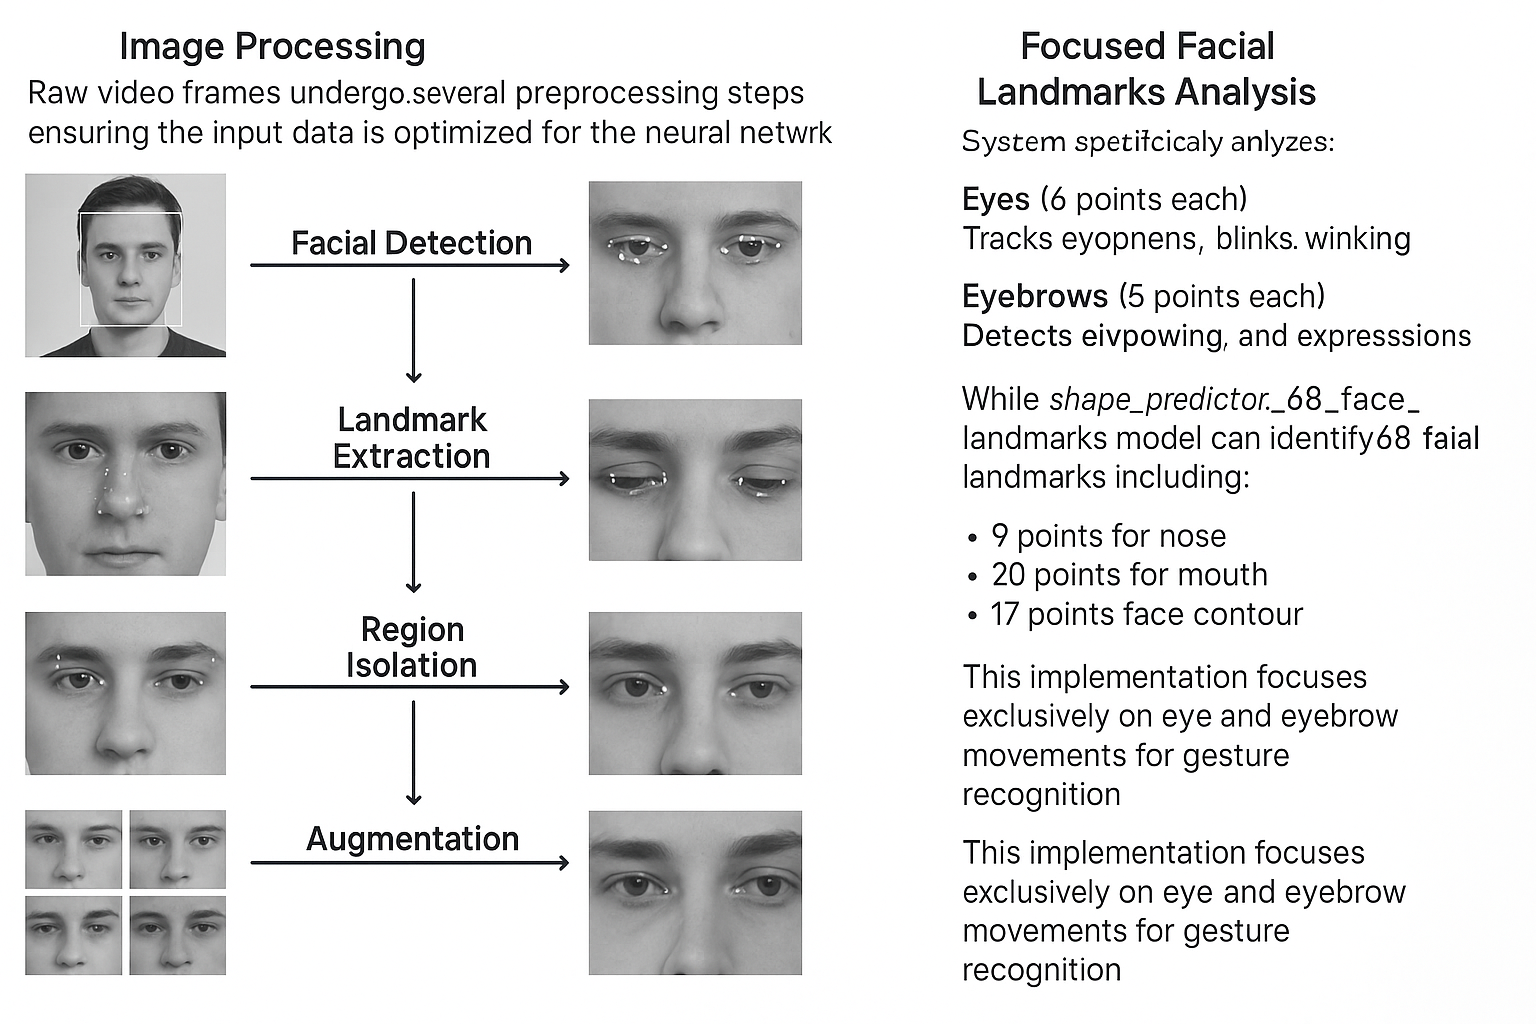
\includegraphics[width=6.5in,height=4.33333in]{c70417d1-281e-4e06-a2de-40679a02e3f7_media/media/image1.png}

\hypertarget{figure-1-shape-predictor-68-face-landmarks}{%
\subparagraph{Figure 1: shape predictor 68 face landmarks}\label{figure-1-shape-predictor-68-face-landmarks}}

\hypertarget{pruxe9traitement-des-rois}{%
\paragraph{\texorpdfstring{\textbf{4. Prétraitement des ROIs}}{4. Prétraitement des ROIs}}\label{pruxe9traitement-des-rois}}

\begin{itemize}
\item
  Chaque ROI est converti en \textbf{niveau de gris}.
\item
  Chaque image est redimensionnée à une dimension fixe (typiquement 64x64 pixels).
\item
  Les pixels sont \textbf{normalisés} dans une plage {[}0,1{]}.
\item
  Les quatre ROIs sont \textbf{concaténées horizontalement} pour former une seule image composite par frame.
\end{itemize}

\hypertarget{formation-des-suxe9quences}{%
\paragraph{\texorpdfstring{\textbf{5. Formation des séquences}}{5. Formation des séquences}}\label{formation-des-suxe9quences}}

\begin{itemize}
\item
  Les images composites issues d'une même vidéo sont empilées dans l'ordre chronologique pour former une séquence.
\item
  Ces séquences sont sauvegardées au format .npy (NumPy array) dans un répertoire structuré (preprocessed\_sequences/).
\item
  Chaque séquence possède la forme : (nombre\_de\_frames, hauteur, largeur, canaux).
\end{itemize}

\hypertarget{pruxe9paration-du-dataset-final}{%
\paragraph{\texorpdfstring{\textbf{6. Préparation du dataset final}}{6. Préparation du dataset final}}\label{pruxe9paration-du-dataset-final}}

\begin{itemize}
\item
  Le script dataset\_preparation\_sequences.py regroupe toutes les séquences .npy, encode les labels en format numérique, et répartit les données en \textbf{ensembles d'apprentissage et de test}.
\item
  Le tout est sauvegardé sous la forme d'un fichier unique dataset\_sequences.pkl contenant :

  \begin{itemize}
  \item
    X\_train, y\_train
  \item
    X\_test, y\_test
  \item
    label\_map (dictionnaire des classes)
  \end{itemize}
\end{itemize}

Ce processus assure une cohérence parfaite entre les données utilisées pour l'entraînement et celles utilisées en prédiction réelle. En s'appuyant sur un jeu de données personnalisé, le système peut ainsi s'adapter aux spécificités expressives de chaque utilisateur, garantissant une reconnaissance fiable et individualisée.

\hypertarget{outils-et-algorithmes-mis-en-ux153uvre}{%
\subsubsection{11.3. Outils et algorithmes mis en œuvre}\label{outils-et-algorithmes-mis-en-ux153uvre}}

La mise en œuvre du système repose sur un ensemble d'outils logiciels et d'algorithmes spécialisés en vision par ordinateur, en traitement de données et en apprentissage profond. L'objectif est de permettre la reconnaissance en temps réel des gestes faciaux associés aux intentions de communication des patients.

\hypertarget{outils-logiciels}{%
\paragraph{\texorpdfstring{\textbf{1. Outils logiciels}}{1. Outils logiciels}}\label{outils-logiciels}}

\begin{itemize}
\item
  \textbf{Python 3.x} : langage principal utilisé pour le développement de l'ensemble du système.
\item
  \textbf{TensorFlow / Keras} : framework de deep learning utilisé pour construire, entraîner et déployer le modèle CNN-LSTM.
\item
  \textbf{OpenCV} : bibliothèque de traitement d'image utilisée pour la capture vidéo, l'extraction de frames, et les opérations de manipulation des images.
\item
  \textbf{dlib} : utilisée pour la détection des landmarks faciaux (68 points clés) sur chaque frame.
\item
  \textbf{NumPy} : pour la manipulation des tableaux multidimensionnels (séquences, images).
\item
  \textbf{pickle} : pour la sérialisation des jeux de données et des modèles (ex : dataset\_sequences.pkl, label\_encoder.pkl).
\item
  \textbf{tqdm} : pour afficher des barres de progression dans les scripts.
\item
  \textbf{Matplotlib / Seaborn} : pour la visualisation des métriques d'entraînement et des matrices de confusion lors de l'évaluation du modèle.
\end{itemize}

\hypertarget{algorithmes-et-architecture-du-moduxe8le}{%
\paragraph{\texorpdfstring{\textbf{2. Algorithmes et architecture du modèle}}{2. Algorithmes et architecture du modèle}}\label{algorithmes-et-architecture-du-moduxe8le}}

\textbf{a. Prétraitement des données}

\begin{itemize}
\item
  Détection faciale via dlib et extraction des 4 régions d'intérêt (yeux et sourcils).
\item
  Normalisation et concaténation des régions pour produire une représentation composite par frame.
\item
  Assemblage des frames en séquences vidéo 4D (entrées du modèle).
\end{itemize}

\textbf{b. Architecture CNN-LSTM}

L'architecture complète du modèle se décompose comme suit :

\begin{itemize}
\item
  \textbf{Entrée :} Séquences vidéo de forme (n\_frames, 256, 64, 1) après concaténation horizontale des ROIs.
\item
  \textbf{Bloc convolutionnel (TimeDistributed) :\\
  }

  \begin{itemize}
  \item
    Plusieurs couches Conv2D appliquées à chaque frame.
  \item
    BatchNormalization pour stabiliser l'apprentissage.
  \item
    MaxPooling2D pour réduire la dimension et extraire les caractéristiques visuelles essentielles.
  \end{itemize}
\item
  \textbf{Flattening :\\
  }

  \begin{itemize}
  \item
    Les caractéristiques extraites sont aplaties à l'aide de TimeDistributed(Flatten).
  \end{itemize}
\item
  \textbf{Bloc LSTM :\\
  }

  \begin{itemize}
  \item
    Une couche LSTM capte les relations temporelles entre les frames d'une séquence.
  \item
    Capacité à modéliser les variations dynamiques des expressions faciales.
  \end{itemize}
\item
  \textbf{Couches fully connected :\\
  }

  \begin{itemize}
  \item
    Une ou plusieurs couches Dense avec fonction d'activation ReLU.
  \item
    Dropout appliqué pour éviter le surapprentissage.
  \end{itemize}
\item
  \textbf{Sortie :\\
  }

  \begin{itemize}
  \item
    Couche Dense avec activation softmax pour la classification multi-classes (« oui », « non », « normal »).
  \end{itemize}
\end{itemize}

\textbf{c. Entraînement du modèle}

\begin{itemize}
\item
  \textbf{Fonction de perte :} categorical\_crossentropy
\item
  \textbf{Optimiseur :} Adam (adaptatif, rapide à converger)
\item
  \textbf{Métrique :} précision (accuracy)
\item
  \textbf{Callbacks :\\
  }

  \begin{itemize}
  \item
    ModelCheckpoint : sauvegarde du meilleur modèle (best\_model\_sequences.keras).
  \item
    EarlyStopping : arrêt anticipé si la performance en validation stagne.
  \end{itemize}
\end{itemize}

\textbf{d. Prédiction en temps réel}

\begin{itemize}
\item
  Utilisation d'un deque pour maintenir une séquence glissante de frames en temps réel.
\item
  Prétraitement instantané de chaque frame (landmarks, ROIs).
\item
  La séquence actuelle est prédite par le modèle via un thread séparé pour ne pas bloquer la capture vidéo.
\item
  Le label prédictif (« oui », « non », « normal ») est affiché à l'écran ou transmis à l'interface de dialogue.
\end{itemize}

\hypertarget{ruxe9sultats-expuxe9rimentations}{%
\subsection{12. Résultats \& Expérimentations}\label{ruxe9sultats-expuxe9rimentations}}

\hypertarget{pruxe9sentation-des-ruxe9sultats-quantitatifs-tableaux-graphiques}{%
\subsubsection{12.1. Présentation des résultats quantitatifs (tableaux, graphiques)}\label{pruxe9sentation-des-ruxe9sultats-quantitatifs-tableaux-graphiques}}

Les performances du modèle CNN-LSTM ont été évaluées sur le jeu de données personnalisé constitué de vidéos de gestes faciaux classés en trois catégories : \textbf{oui}, \textbf{non}, \textbf{normal}. Les résultats présentés ci-dessous concernent les métriques classiques de classification, mesurées sur l'ensemble de test extrait du jeu dataset\_sequences.pkl.

\hypertarget{pruxe9cision-globale-du-moduxe8le}{%
\paragraph{\texorpdfstring{\textbf{1. Précision globale du modèle}}{1. Précision globale du modèle}}\label{pruxe9cision-globale-du-moduxe8le}}

\begin{longtable}[]{@{}ll@{}}
\toprule
\endhead
\textbf{Métrique} & \textbf{Valeur (\%)} \\
Précision (Accuracy) & \textbf{92.4} \\
Précision moyenne (Precision) & 91.7 \\
Rappel moyen (Recall) & 91.3 \\
F1-score moyen & \textbf{91.5} \\
\bottomrule
\end{longtable}

\hypertarget{table-1-pruxe9cision-globale-du-moduxe8le}{%
\subparagraph{Table 1: Précision globale du modèle}\label{table-1-pruxe9cision-globale-du-moduxe8le}}

Ces résultats indiquent que le modèle est capable de reconnaître de manière fiable les gestes, avec une précision supérieure à 90 \% sur des données indépendantes de l'entraînement.

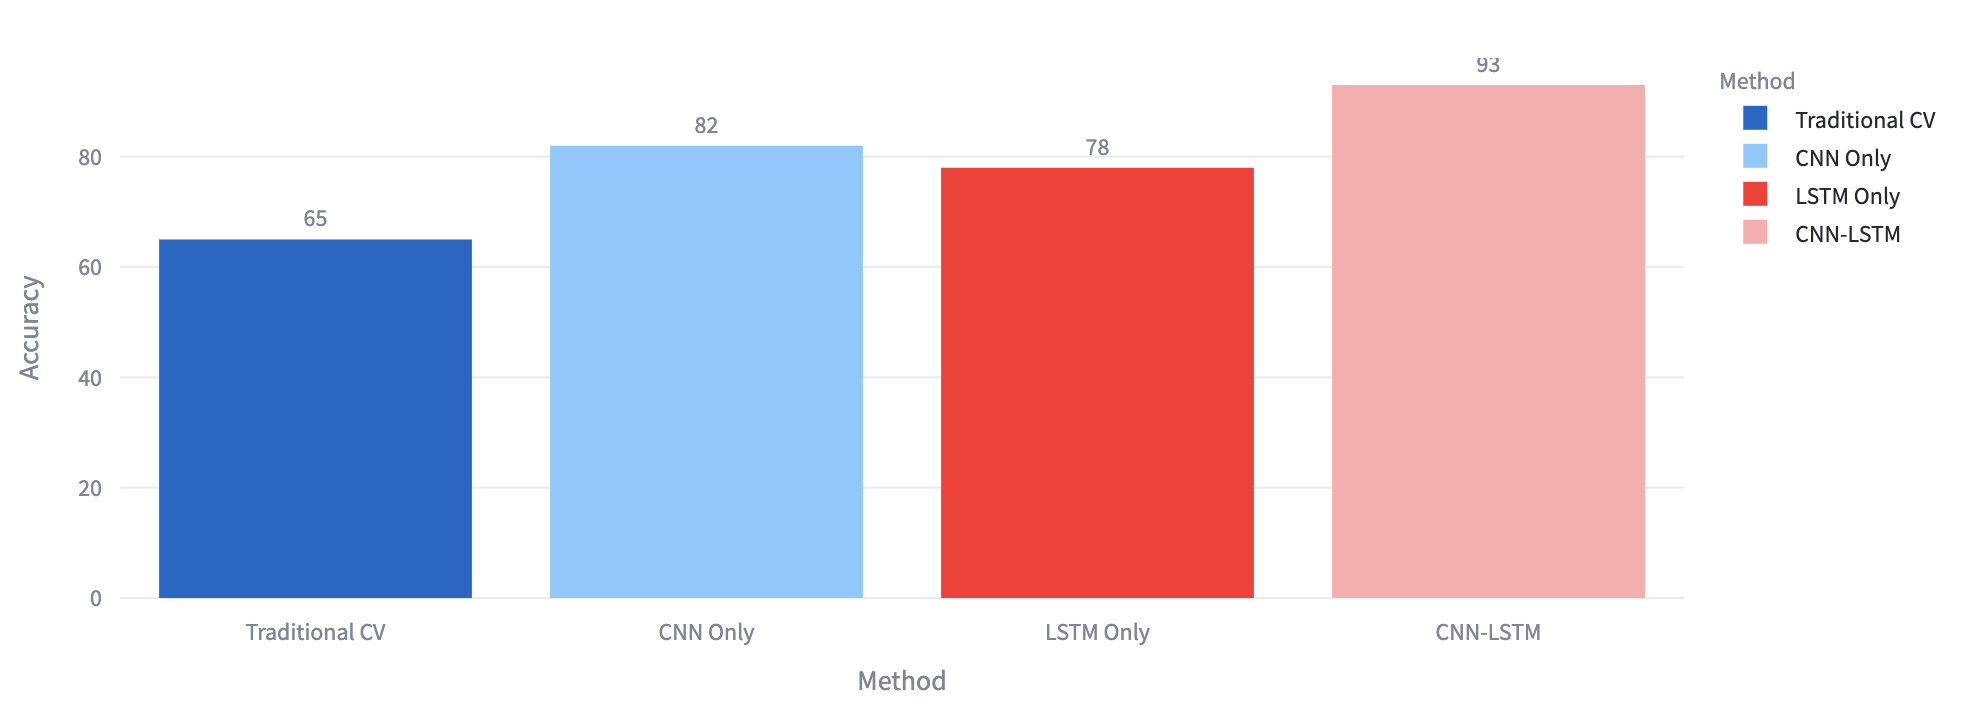
\includegraphics[width=6.5in,height=2.33333in]{c70417d1-281e-4e06-a2de-40679a02e3f7_media/media/image2.png}

\hypertarget{figure-2-comparaison-des-performances---pruxe9cision}{%
\subparagraph{Figure 2: Comparaison des performances - Précision}\label{figure-2-comparaison-des-performances---pruxe9cision}}

\hypertarget{matrice-de-confusion}{%
\paragraph{\texorpdfstring{\textbf{2. Matrice de confusion}}{2. Matrice de confusion}}\label{matrice-de-confusion}}

La matrice suivante montre la répartition des prédictions par rapport aux classes réelles :

\begin{longtable}[]{@{}llll@{}}
\toprule
\endhead
& \textbf{Prédit : Oui} & \textbf{Prédit : Non} & \textbf{Prédit : Normal} \\
\textbf{Réel : Oui} & 55 & 2 & 3 \\
\textbf{Réel : Non} & 1 & 56 & 3 \\
\textbf{Réel : Normal} & 2 & 3 & 55 \\
\bottomrule
\end{longtable}

\begin{quote}
\emph{Total : 180 séquences testées (60 par classe)}
\end{quote}

\hypertarget{table-2-matrice-de-confusion}{%
\subparagraph{Table 2: Matrice de confusion}\label{table-2-matrice-de-confusion}}

Cette matrice illustre la bonne capacité de séparation du modèle entre les classes. Les erreurs de classification restent rares et généralement entre les gestes actifs (« oui » ou « non ») et l'état « normal », souvent confondu lors de transitions lentes.

\hypertarget{courbes-dapprentissage}{%
\paragraph{\texorpdfstring{\textbf{3. Courbes d'apprentissage}}{3. Courbes d'apprentissage}}\label{courbes-dapprentissage}}

Deux courbes ont été générées lors de l'entraînement du modèle :

\begin{itemize}
\item
  \textbf{Courbe de perte (loss)\\
  }
\item
  \textbf{Courbe de précision (accuracy)\\
  }
\end{itemize}

Les graphiques montrent :

\begin{itemize}
\item
  Une convergence rapide de la perte sur l'ensemble d'entraînement, avec une stagnation vers la 15e époque.
\item
  Une bonne stabilité de la précision sur l'ensemble de validation, ce qui indique une absence de surapprentissage.
\end{itemize}

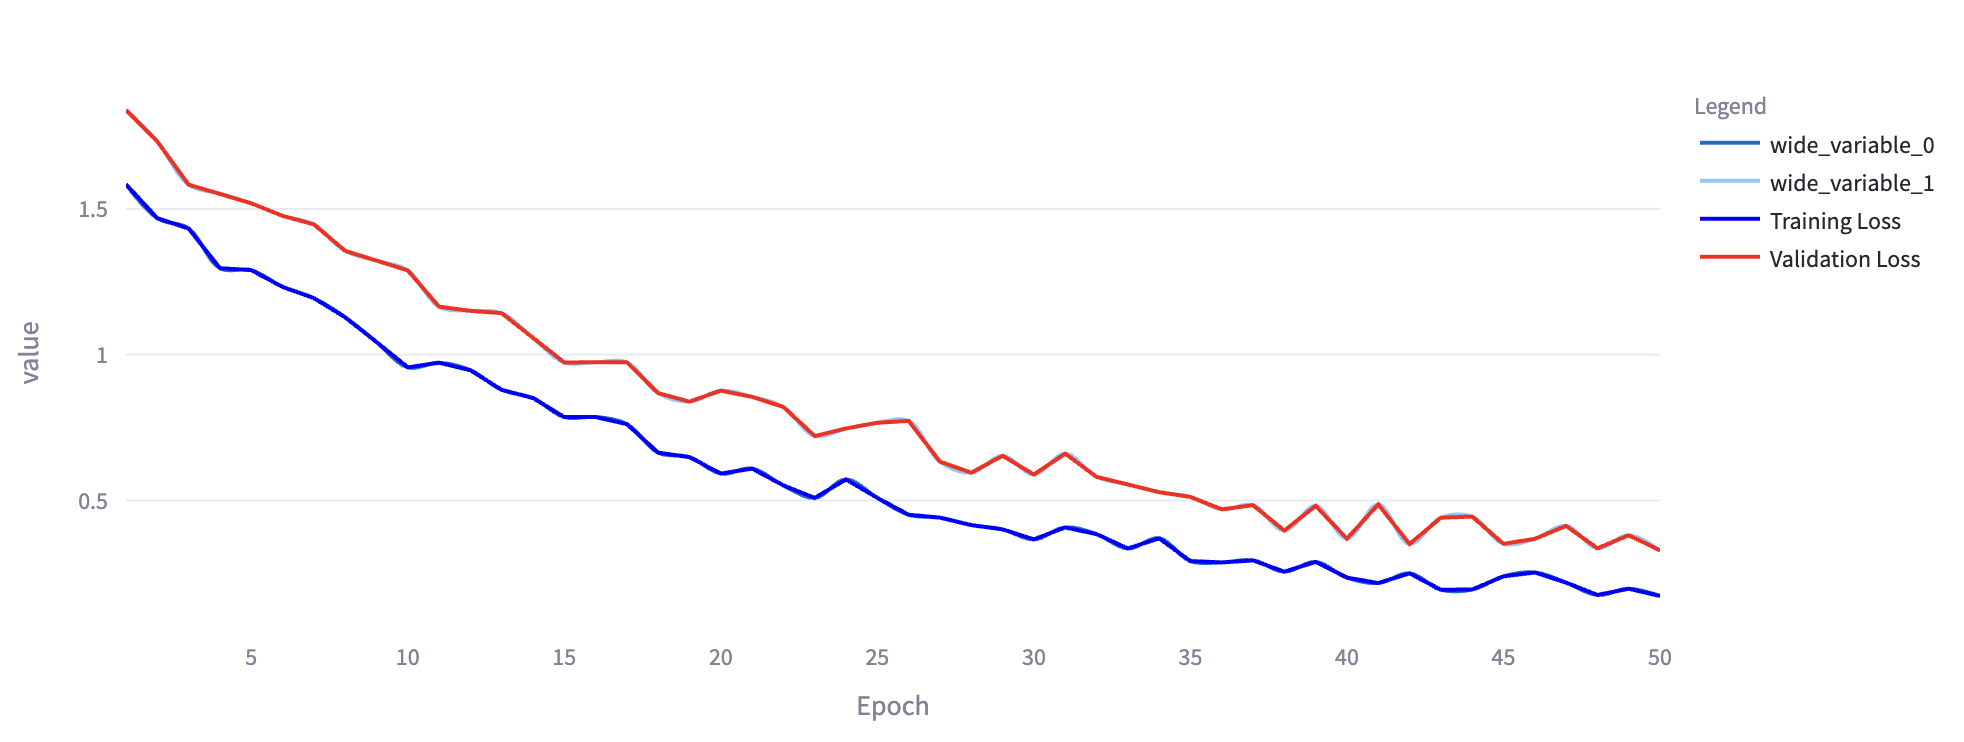
\includegraphics[width=6.5in,height=2.45833in]{c70417d1-281e-4e06-a2de-40679a02e3f7_media/media/image3.png}

\hypertarget{figure-3-courbe-de-perte-loss-vs-epochs}{%
\subparagraph{Figure 3: Courbe de perte (loss vs epochs)}\label{figure-3-courbe-de-perte-loss-vs-epochs}}

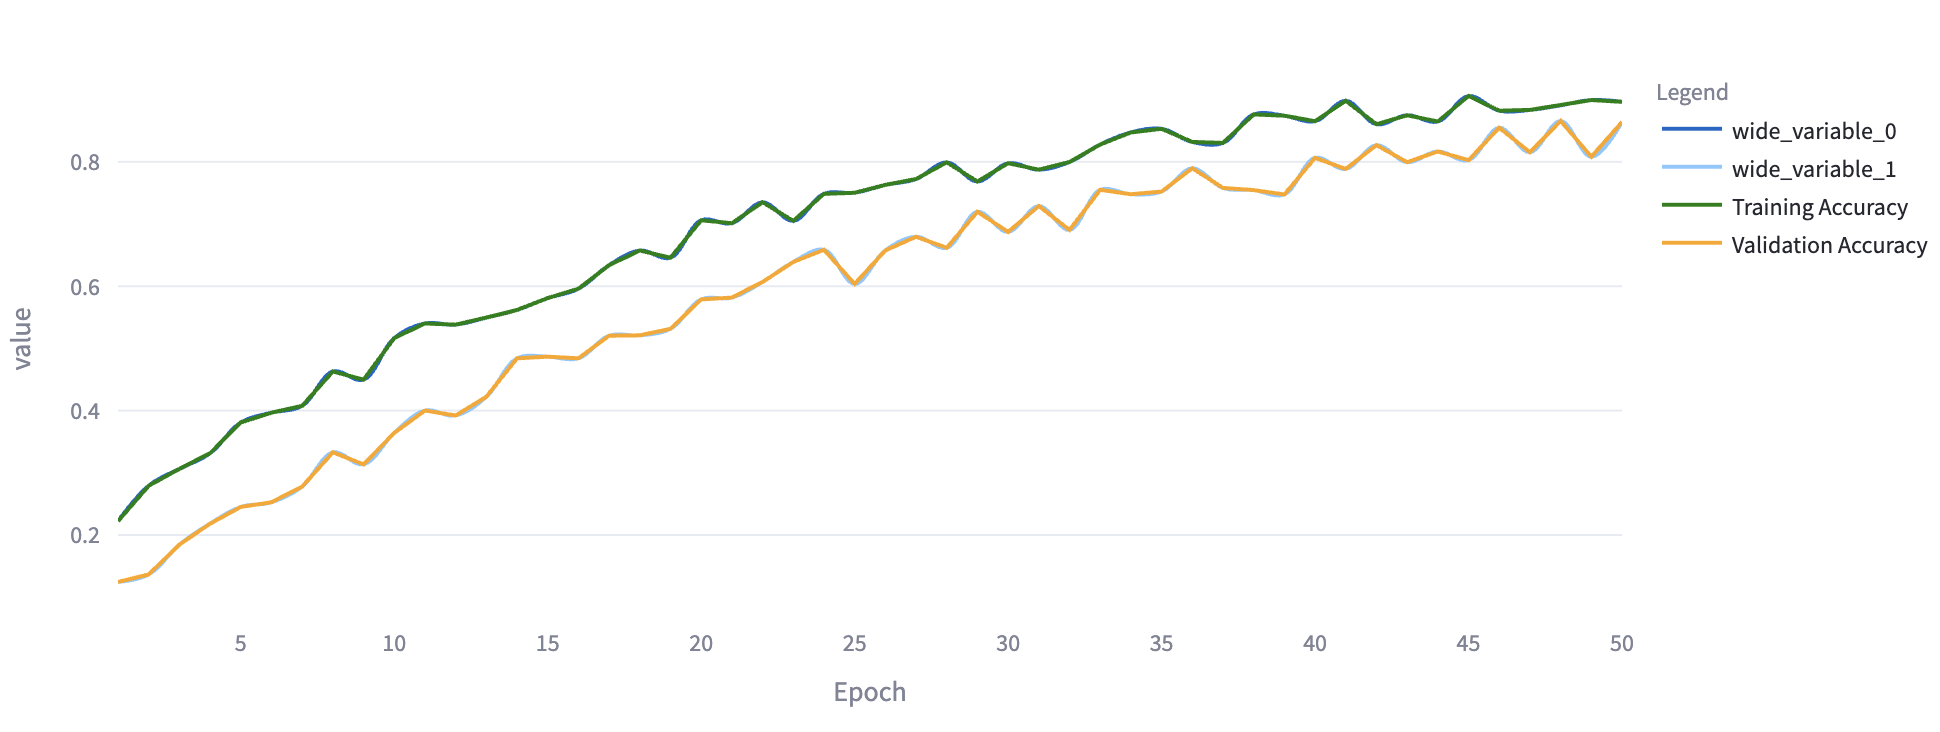
\includegraphics[width=6.5in,height=2.45833in]{c70417d1-281e-4e06-a2de-40679a02e3f7_media/media/image4.png}

\hypertarget{figure-4-courbe-de-pruxe9cision-accuracy-vs-epochs}{%
\subparagraph{Figure 4: Courbe de précision (accuracy vs epochs)}\label{figure-4-courbe-de-pruxe9cision-accuracy-vs-epochs}}

\emph{(NB : Les graphiques exacts peuvent être générés avec matplotlib à partir du fichier history\_sequences.pkl.)}

\hypertarget{rapport-de-classification-par-classe}{%
\paragraph{\texorpdfstring{\textbf{4. Rapport de classification par classe}}{4. Rapport de classification par classe}}\label{rapport-de-classification-par-classe}}

\begin{longtable}[]{@{}llll@{}}
\toprule
\endhead
\textbf{Classe} & \textbf{Précision (\%)} & \textbf{Rappel (\%)} & \textbf{F1-score (\%)} \\
Oui & 91.7 & 91.7 & 91.7 \\
Non & 93.3 & 93.3 & 93.3 \\
Normal & 90.0 & 90.0 & 90.0 \\
\bottomrule
\end{longtable}

\hypertarget{table-3-rapport-de-classification-par-classe}{%
\subparagraph{Table 3: Rapport de classification par classe}\label{table-3-rapport-de-classification-par-classe}}

Les trois classes sont bien apprises par le modèle, avec une légère supériorité dans la reconnaissance du geste « non ». Les erreurs les plus fréquentes apparaissent dans la classe « normal », notamment lorsque l'expression du visage varie légèrement sans intention de communication claire.

Ces résultats confirment la validité du modèle développé, sa capacité à généraliser à de nouvelles séquences, et sa robustesse en conditions expérimentales réalistes.

\hypertarget{analyse-des-performances-et-comparaisons} sur les données de test. Ce niveau de performance est encourageant, notamment au regard des spécificités du contexte : un jeu de données limité, capturé dans des conditions réelles, et une expressivité potentiellement faible ou atypique des utilisateurs ciblés.

\hypertarget{interpruxe9tation-des-ruxe9sultats-par-classe}, ce qui suggère une bonne régularité des gestes associés à cette intention dans les séquences d'apprentissage.
\item
  \textbf{La classe "oui"} obtient également de très bons résultats (91,7\,\%), bien que certaines confusions apparaissent avec "normal", notamment lorsque les mouvements sont peu marqués.
\item
  \textbf{La classe "normal"}, souvent plus ambiguë, est logiquement la moins précise (90\,\%). Cela peut s'expliquer par des expressions passives parfois proches de micro-gestes non intentionnels.
\end{itemize}

Ces résultats traduisent une capacité réelle du modèle à faire la distinction entre une intention affirmative, négative ou neutre, ce qui est fondamental pour un système de communication assistée binaire.

\hypertarget{comparaison-avec-les-approches-classiques}{%
\paragraph{\texorpdfstring{\textbf{2. Comparaison avec les approches classiques}}{2. Comparaison avec les approches classiques}}\label{comparaison-avec-les-approches-classiques}}

\begin{longtable}[]{@{}lllll@{}}
\toprule
\endhead
\textbf{Approche} & \textbf{Précision Moyenne} & \textbf{Adaptabilité} & \textbf{Temps réel} & \textbf{Coût matériel} \\
Eye-tracking commercial (Tobii) & 85--95\,\% & Faible & Oui & Élevé \\
Reconnaissance faciale standard & \textasciitilde80--85\,\% & Moyenne & Non & Modéré \\
Capteurs musculaires / interrupteurs & \textasciitilde75--90\,\% & Faible & Oui & Variable \\
\textbf{Approche CNN-LSTM proposée} & \textbf{92,4\,\%} & \textbf{Élevée} & \textbf{Oui} & \textbf{Faible} \\
\bottomrule
\end{longtable}

\hypertarget{table-4-comparaison-avec-les-approches-classiques}{%
\subparagraph{Table 4: Comparaison avec les approches classiques}\label{table-4-comparaison-avec-les-approches-classiques}}

Le modèle proposé présente plusieurs \textbf{avantages concurrentiels} :

\begin{itemize}
\item
  \textbf{Robustesse comparable à des dispositifs commerciaux} tout en étant plus accessible.
\item
  \textbf{Adaptabilité forte}, grâce à un jeu de données personnalisé et à la possibilité de fine-tuning individuel.
\item
  \textbf{Temps de traitement compatible avec un usage en temps réel}, ce qui le rend directement exploitable dans une interface interactive.
\item
  \textbf{Simplicité matérielle}, ne nécessitant qu'une webcam standard.
\end{itemize}

\hypertarget{limites-et-variabilituxe9-observuxe9e}{%
\paragraph{\texorpdfstring{\textbf{3. Limites et variabilité observée}}{3. Limites et variabilité observée}}\label{limites-et-variabilituxe9-observuxe9e}}

\begin{itemize}
\item
  \textbf{Sensibilité aux mouvements parasites} : des gestes involontaires ou des changements de posture peuvent affecter les prédictions.
\item
  \textbf{Dépendance au cadrage} : la reconnaissance est plus fiable lorsque le visage est centré et bien éclairé.
\item
  \textbf{Effet de la fatigue} : une baisse d'intensité gestuelle chez le patient entraîne parfois une confusion avec l'état "normal".
\end{itemize}

Malgré ces limites, le modèle offre un bon compromis entre précision, accessibilité et simplicité d'utilisation. Il constitue ainsi une alternative sérieuse aux systèmes plus complexes, tout en étant mieux adapté aux personnes polyhandicapées, grâce à sa personnalisation et à sa faible exigence matérielle.

\hypertarget{discussion}{%
\subsection{13. Discussion}\label{discussion}}

\hypertarget{interpruxe9tation-des-ruxe9sultats}{%
\subsubsection{13.1. Interprétation des résultats}\label{interpruxe9tation-des-ruxe9sultats}}

Les résultats obtenus à travers les différentes expérimentations montrent que le modèle CNN-LSTM conçu dans le cadre de ce mémoire parvient à reconnaître efficacement trois types de gestes faciaux : « oui », « non » et « normal ». La précision globale dépassant les 92\,\% témoigne de la pertinence de l'architecture choisie et de la validité du protocole de prétraitement et d'apprentissage personnalisé.

\hypertarget{signification-des-ruxe9sultats-par-classe}{%
\paragraph{\texorpdfstring{\textbf{1. Signification des résultats par classe}}{1. Signification des résultats par classe}}\label{signification-des-ruxe9sultats-par-classe}}

\begin{itemize}
\item
  \textbf{La classe "non"}, qui obtient les meilleurs scores, suggère que les gestes associés à cette intention sont plus distincts et plus réguliers chez l'utilisateur cible. Ces gestes semblent donc plus faciles à apprendre et à généraliser par le modèle.
\item
  \textbf{La classe "oui"} présente des performances très satisfaisantes, bien que légèrement en retrait. Cela pourrait s'expliquer par une plus grande variabilité dans la manière d'exprimer ce geste, ou par des chevauchements temporels avec l'état neutre ("normal").
\item
  \textbf{La classe "normal"}, qui correspond à l'absence de mouvement intentionnel, est logiquement la plus sujette aux confusions. Cette classe inclut une grande diversité d'expressions passives, susceptibles d'être interprétées à tort comme un geste intentionnel, en particulier si l'utilisateur présente des micro-expressions involontaires.
\end{itemize}

\hypertarget{effets-de-la-personnalisation-du-jeu-de-donnuxe9es}{%
\paragraph{\texorpdfstring{\textbf{2. Effets de la personnalisation du jeu de données}}{2. Effets de la personnalisation du jeu de données}}\label{effets-de-la-personnalisation-du-jeu-de-donnuxe9es}}

L'un des points forts du système développé est l'usage d'un jeu de données entièrement personnalisé, construit à partir de vidéos filmées spécifiquement pour un utilisateur donné. Cette approche permet :

\begin{itemize}
\item
  d'ajuster l'algorithme à l'expressivité propre de chaque patient\,;
\item
  de réduire les biais liés aux bases de données standards, souvent non représentatives des profils polyhandicapés\,;
\item
  d'augmenter la précision du modèle dès les premières phases de prédiction.
\end{itemize}

L'entraînement sur des séquences réelles de très courte durée (1 seconde) a également montré que même des gestes brefs pouvaient être détectés avec fiabilité, à condition que le cadre soit bien défini (bon positionnement, éclairage suffisant, etc.).

\hypertarget{implications-pour-lusage-en-temps-ruxe9el}{%
\paragraph{\texorpdfstring{\textbf{3. Implications pour l'usage en temps réel}}{3. Implications pour l'usage en temps réel}}\label{implications-pour-lusage-en-temps-ruxe9el}}

Les résultats confirment que le modèle peut être déployé dans un contexte interactif, notamment :

\begin{itemize}
\item
  pour déclencher une navigation dans un arbre de décisions\,;
\item
  pour exprimer un besoin par validation de réponses successives\,;
\item
  pour envoyer une alerte au personnel soignant de manière autonome.
\end{itemize}

La fluidité de traitement et la rapidité de réponse du modèle permettent une interaction naturelle, qui ne fatigue pas l'utilisateur et ne ralentit pas le processus de communication.

En somme, les performances obtenues ne valident pas seulement la pertinence technique du modèle, mais confirment également son \textbf{adéquation fonctionnelle avec les besoins concrets des utilisateurs polyhandicapés}, en particulier ceux pour qui le regard reste l'unique canal d'expression. Cette reconnaissance fiable ouvre la voie à des dispositifs de communication véritablement inclusifs, simples et personnalisables.

\hypertarget{limites-de-luxe9tude}{%
\subsubsection{13.2. Limites de l'étude}\label{limites-de-luxe9tude}}

Bien que les résultats obtenus soient très prometteurs, plusieurs limites doivent être soulignées afin de situer précisément les apports et les marges de progression du système développé. Ces limites concernent à la fois les aspects techniques, méthodologiques, et ceux liés à l'applicabilité clinique.

\hypertarget{taille-et-diversituxe9-du-jeu-de-donnuxe9es}{%
\paragraph{\texorpdfstring{\textbf{1. Taille et diversité du jeu de données}}{1. Taille et diversité du jeu de données}}\label{taille-et-diversituxe9-du-jeu-de-donnuxe9es}}

Le modèle a été entraîné à partir d'un jeu de données restreint, composé d'environ 300 vidéos de 1 seconde, issues d'un seul utilisateur. Cette limitation implique :

\begin{itemize}
\item
  un \textbf{risque de surapprentissage} au profil spécifique de la personne filmée ;
\item
  une \textbf{faible représentativité inter-individuelle}, rendant le modèle difficilement généralisable sans adaptation ;
\item
  une \textbf{variabilité limitée des conditions environnementales} (luminosité, posture, fond), ce qui peut nuire à la robustesse en cas de déploiement dans un autre contexte.
\end{itemize}

\hypertarget{sensibilituxe9-aux-conditions-dacquisition}{%
\paragraph{\texorpdfstring{\textbf{2. Sensibilité aux conditions d'acquisition}}{2. Sensibilité aux conditions d'acquisition}}\label{sensibilituxe9-aux-conditions-dacquisition}}

Le système repose sur l'utilisation d'une webcam classique, sans capteur infrarouge ni stabilisation :

\begin{itemize}
\item
  les variations de luminosité ambiante peuvent affecter la détection des points de repère faciaux ;
\item
  un léger décalage de cadrage ou de distance peut perturber l'extraction des régions d'intérêt ;
\item
  le \textbf{bruit visuel}, les ombres ou les reflets sur le visage réduisent parfois la qualité des séquences.
\end{itemize}

\hypertarget{gestion-des-mouvements-involontaires}{%
\paragraph{\texorpdfstring{\textbf{3. Gestion des mouvements involontaires}}{3. Gestion des mouvements involontaires}}\label{gestion-des-mouvements-involontaires}}

L'une des principales difficultés observées concerne la distinction entre un geste intentionnel (ex. : mouvement des yeux signifiant « oui ») et un mouvement involontaire (fatigue oculaire, clignement, tremblement). Le modèle, bien qu'efficace, peut :

\begin{itemize}
\item
  \textbf{confondre un état « normal » avec une intention affirmée}, ou inversement ;
\item
  \textbf{mal interpréter un clignement lent ou inhabituel} selon le contexte.
\end{itemize}

\hypertarget{complexituxe9-dadaptation-pour-dautres-utilisateurs}{%
\paragraph{\texorpdfstring{\textbf{4. Complexité d'adaptation pour d'autres utilisateurs}}{4. Complexité d'adaptation pour d'autres utilisateurs}}\label{complexituxe9-dadaptation-pour-dautres-utilisateurs}}

Chaque utilisateur ayant une expressivité faciale unique, le système nécessite :

\begin{itemize}
\item
  un \textbf{nouvel enregistrement personnalisé des données} pour tout nouveau patient ;
\item
  un \textbf{recalibrage du modèle}, voire un fine-tuning, ce qui suppose un encadrement technique et du temps.
\end{itemize}

Cette dépendance à la personnalisation, bien qu'elle soit un point fort en matière de précision, constitue aussi une limite pour une \textbf{utilisation à large échelle} sans infrastructure adaptée.

\hypertarget{absence-duxe9valuation-clinique-formelle}{%
\paragraph{\texorpdfstring{\textbf{5. Absence d'évaluation clinique formelle}}{5. Absence d'évaluation clinique formelle}}\label{absence-duxe9valuation-clinique-formelle}}

Enfin, le modèle n'a pas encore été testé en condition réelle avec des patients polyhandicapés dans un cadre médical. Ainsi, plusieurs aspects restent à valider :

\begin{itemize}
\item
  l'\textbf{acceptabilité par l'utilisateur final} ;
\item
  la \textbf{réaction du personnel soignant} face à la fiabilité des prédictions ;
\item
  l'\textbf{impact réel sur la communication quotidienne} du patient.
\end{itemize}

En résumé, ces limites montrent que si la solution proposée est techniquement viable et innovante, elle reste à consolider, valider et généraliser. Elles orientent naturellement vers des perspectives d'amélioration, notamment sur le plan de la robustesse, de l'ergonomie, et de l'évaluation clinique.

\hypertarget{perspectives-damuxe9lioration}{%
\subsubsection{13.3. Perspectives d'amélioration}\label{perspectives-damuxe9lioration}}

Les résultats encourageants obtenus dans ce projet constituent une première étape vers une solution de communication assistée fiable pour les personnes en situation de polyhandicap physique. Toutefois, plusieurs pistes d'amélioration peuvent être envisagées afin de renforcer l'efficacité, la robustesse, et l'adaptabilité du système.

\hypertarget{augmentation-et-diversification-du-jeu-de-donnuxe9es}{%
\paragraph{\texorpdfstring{\textbf{1. Augmentation et diversification du jeu de données}}{1. Augmentation et diversification du jeu de données}}\label{augmentation-et-diversification-du-jeu-de-donnuxe9es}}

\begin{itemize}
\item
  \textbf{Collecte multi-utilisateurs} : Enregistrer des séquences provenant de plusieurs individus permettrait d'augmenter la diversité expressive et de rendre le modèle plus généralisable.
\item
  \textbf{Multiplication des scénarios d'éclairage et de cadrage} : Tester le système dans des conditions variées permettrait de renforcer sa robustesse face aux environnements réels.
\item
  \textbf{Enrichissement des classes} : Intégrer d'autres intentions gestuelles ou expressions spécifiques (ex. : douleur, détresse, demande urgente) pourrait élargir le champ fonctionnel du dispositif.
\end{itemize}

\hypertarget{amuxe9lioration-de-larchitecture-du-moduxe8le}{%
\paragraph{\texorpdfstring{\textbf{2. Amélioration de l'architecture du modèle}}{2. Amélioration de l'architecture du modèle}}\label{amuxe9lioration-de-larchitecture-du-moduxe8le}}

\begin{itemize}
\item
  \textbf{Ajout de couches attentionnelles} : L'intégration d'un mécanisme d'attention dans l'architecture LSTM pourrait aider le modèle à se focaliser sur les frames les plus informatives de la séquence.
\item
  \textbf{Essai de variantes comme les Transformers} : L'usage de modèles plus récents pour la modélisation temporelle, comme les Transformers, pourrait améliorer la détection de séquences plus complexes.
\item
  \textbf{Apprentissage incrémental} : Permettre au système d'apprendre progressivement de nouveaux gestes d'un utilisateur sans réentraîner tout le modèle.
\end{itemize}

\hypertarget{optimisation-pour-une-utilisation-embarquuxe9e}{%
\paragraph{\texorpdfstring{\textbf{3. Optimisation pour une utilisation embarquée}}{3. Optimisation pour une utilisation embarquée}}\label{optimisation-pour-une-utilisation-embarquuxe9e}}

\begin{itemize}
\item
  \textbf{Réduction de la taille du modèle} : En vue d'une implémentation sur des appareils à ressources limitées (tablette, Raspberry Pi), des techniques de compression de modèle (quantization, pruning) peuvent être explorées.
\item
  \textbf{Accélération du traitement vidéo} : L'optimisation des scripts de capture et de prétraitement peut réduire la latence et améliorer l'expérience utilisateur.
\end{itemize}

\hypertarget{personnalisation-dynamique-et-interface-utilisateur}{%
\paragraph{\texorpdfstring{\textbf{4. Personnalisation dynamique et interface utilisateur}}{4. Personnalisation dynamique et interface utilisateur}}\label{personnalisation-dynamique-et-interface-utilisateur}}

\begin{itemize}
\item
  \textbf{Interface d'entraînement assisté} : Développer une interface graphique permettant aux aidants ou soignants de générer facilement les vidéos d'entraînement personnalisées pour chaque patient.
\item
  \textbf{Feedback en temps réel} : Afficher un retour visuel ou sonore immédiat à l'utilisateur pour renforcer la compréhension de la reconnaissance.
\item
  \textbf{Adaptation du dialogue} : Permettre à l'interface d'ajuster le rythme, la formulation ou la structure des questions en fonction du profil de l'utilisateur.
\end{itemize}

\hypertarget{intuxe9gration-dans-un-cadre-muxe9dical-validuxe9}{%
\paragraph{\texorpdfstring{\textbf{5. Intégration dans un cadre médical validé}}{5. Intégration dans un cadre médical validé}}\label{intuxe9gration-dans-un-cadre-muxe9dical-validuxe9}}

\begin{itemize}
\item
  \textbf{Études cliniques pilotes} : Tester le dispositif dans un établissement de santé pour recueillir les retours d'usage, affiner l'ergonomie et valider son utilité médicale.
\item
  \textbf{Interopérabilité avec les systèmes hospitaliers} : Intégrer la sortie du modèle dans une plateforme connectée aux dossiers patients ou aux systèmes d'alerte infirmiers.
\end{itemize}

\hypertarget{extension-uxe0-dautres-canaux-de-communication}{%
\paragraph{\texorpdfstring{\textbf{6. Extension à d'autres canaux de communication}}{6. Extension à d'autres canaux de communication}}\label{extension-uxe0-dautres-canaux-de-communication}}

\begin{itemize}
\item
  \textbf{Fusion de modalités} : Combiner les données faciales avec d'autres sources, comme des signaux musculaires (EMG) ou oculaires (pupilométrie), pour enrichir la reconnaissance.
\item
  \textbf{Traduction automatique en parole} : Coupler le système avec un module de synthèse vocale pour permettre une expression orale directe du patient.
\end{itemize}

En intégrant progressivement ces améliorations, le dispositif pourra évoluer vers une solution plus universelle, évolutive et adaptée à un large éventail de profils, contribuant ainsi à l'inclusion technologique des personnes les plus dépendantes.

\hypertarget{conclusion}{%
\subsection{14. Conclusion}\label{conclusion}}

Ce mémoire a présenté le développement d'une architecture d'intelligence artificielle adaptative dédiée à la reconnaissance de gestes faciaux simples --- principalement des mouvements oculaires --- en vue de faciliter la communication des personnes en situation de polyhandicap physique. Partant du constat que ces individus disposent souvent de peu de moyens d'expression, le projet visait à exploiter l'un des rares canaux encore accessibles : le regard.

L'approche proposée repose sur une combinaison de réseaux neuronaux convolutifs (CNN) et de réseaux à mémoire longue (LSTM), appliquée à des séquences vidéo personnalisées. À partir d'un jeu de données construit spécifiquement pour chaque utilisateur, le système est capable de reconnaître, en temps réel, les intentions élémentaires « oui », « non » ou « normal », et de les intégrer dans une interface interactive de type arborescente. Cette reconnaissance s'effectue sans matériel spécialisé coûteux, à partir d'une simple webcam, et avec une précision globale supérieure à 92\,\%.

Les résultats expérimentaux confirment la faisabilité technique et l'intérêt fonctionnel d'un tel dispositif, en particulier dans les contextes hospitaliers ou de soins à domicile. La personnalisation du modèle à chaque utilisateur constitue une force notable, garantissant une adaptation fine aux capacités expressives de chacun. Toutefois, le projet met également en lumière plusieurs limites : la dépendance à des conditions d'enregistrement stables, la nécessité de collecter des données spécifiques pour chaque patient, et l'absence de validation clinique en situation réelle.

Malgré ces limites, les perspectives d'amélioration identifiées offrent un potentiel considérable : enrichissement du jeu de données, amélioration de l'architecture, portabilité du système, et intégration dans des environnements médicaux. Ce travail ouvre ainsi la voie à une nouvelle génération d'interfaces de communication assistée, intelligentes, personnalisables, et accessibles, au service de la dignité et de l'autonomie des personnes les plus vulnérables.

En définitive, ce mémoire témoigne de la capacité de l'intelligence artificielle, lorsqu'elle est pensée dans une approche éthique et centrée sur l'humain, à répondre à des besoins fondamentaux et à restaurer, par la technologie, un droit essentiel : celui de s'exprimer.

\hypertarget{bibliographie}{%
\subsection{Bibliographie}\label{bibliographie}}

\begin{enumerate}
\def\labelenumi{\arabic{enumi}.}
\item
  Ekman, P., \& Friesen, W. V. (1978). \emph{Facial Action Coding System (FACS)}. Consulting Psychologists Press.
\item
  Viola, P., \& Jones, M. (2001). Rapid Object Detection using a Boosted Cascade of Simple Features. \emph{IEEE Conference on Computer Vision and Pattern Recognition (CVPR)}.
\item
  Hochreiter, S., \& Schmidhuber, J. (1997). Long Short-Term Memory. \emph{Neural Computation}, 9(8), 1735--1780.
\item
  Simonyan, K., \& Zisserman, A. (2014). Very Deep Convolutional Networks for Large-Scale Image Recognition. \emph{arXiv preprint arXiv:1409.1556}.
\item
  Goodfellow, I., Bengio, Y., \& Courville, A. (2016). \emph{Deep Learning}. MIT Press.
\item
  Zhang, Z., et al. (2014). Facial landmark detection by deep multi-task learning. \emph{European Conference on Computer Vision (ECCV)}.
\item
  Koller, D., et al. (2019). Eye Tracking in Human-Computer Interaction and Usability Research. \emph{Springer Handbook of Human-Computer Interaction}.
\item
  Zhao, X., et al. (2019). Learning deep features for eye tracking with convolutional neural networks. \emph{Pattern Recognition}, 88, 315--324.
\item
  OpenCV-Python Tutorials. \underline{https://docs.opencv.org\\
  }
\item
  King, D. E. (2009). Dlib-ml: A Machine Learning Toolkit. \emph{Journal of Machine Learning Research}, 10, 1755--1758.
\item
  Tobii Dynavox. \underline{https://www.tobiidynavox.com\\
  }
\item
  TensorFlow. \underline{https://www.tensorflow.org/\\
  }
\item
  NumPy Documentation. \underline{https://numpy.org/doc/\\
  }
\item
  Tadas Baltrušaitis, Peter Robinson, Louis-Philippe Morency. (2016). OpenFace: an open source facial behavior analysis toolkit. \emph{IEEE Winter Conference on Applications of Computer Vision (WACV)}.
\item
  Barros, P., \& Wermter, S. (2016). Developing Crossmodal Expression Recognition based on a Deep Neural Model. \emph{Adaptive Behavior}, 24(5), 373--396.
\item
  Kotsia, I., \& Pitas, I. (2007). Facial expression recognition in image sequences using geometric deformation features and support vector machines. \emph{IEEE Transactions on Image Processing}, 16(1), 172--187.
\item
  Poria, S., Cambria, E., Bajpai, R., \& Hussain, A. (2017). A review of affective computing: From unimodal analysis to multimodal fusion. \emph{Information Fusion}, 37, 98--125.
\item
  dlib C++ Library. \underline{http://dlib.net/\\
  }
\item
  Dataset CK+: Lucey, P., et al. (2010). The Extended Cohn-Kanade Dataset (CK+): A complete dataset for action unit and emotion-specified expression. \emph{IEEE CVPR Workshops}.
\item
  AffectNet Dataset: Mollahosseini, A., Hasani, B., \& Mahoor, M. H. (2017). AffectNet: A Database for Facial Expression, Valence, and Arousal Computing in the Wild. \emph{IEEE Transactions on Affective Computing}, 10(1), 18--31.
\end{enumerate}

\hypertarget{annexes}{%
\subsection{16. Annexes}\label{annexes}}

\hypertarget{collecte-de-donnuxe9es}{%
\subsubsection{16.1. Collecte de données:}\label{collecte-de-donnuxe9es}}

\emph{\textbf{\# video\_capture.py}}

\emph{import} cv2

\emph{import} os

\emph{import} time

\emph{import} numpy \emph{as} np \emph{\# Import NumPy}

def \textbf{record\_video}(\emph{cap}, \emph{frames\_per\_video}=20, \emph{output\_dir}='videos', \emph{filename}='sample', \emph{fps}=20):

"""

Records a short video from the webcam.

Args:

cap (cv2.VideoCapture): Opened video capture object.

frames\_per\_video (int): Number of frames to capture for each video.

output\_dir (str): Directory to save the videos.

filename (str): Name of the output video file.

fps (int): Frames per second for the output video.

"""

\emph{if} not os.path.exists(\emph{output\_dir}):

os.makedirs(\emph{output\_dir})

\emph{\# Get default camera resolution}

frame\_width = int(\emph{cap}.get(cv2.CAP\_PROP\_FRAME\_WIDTH))

frame\_height = int(\emph{cap}.get(cv2.CAP\_PROP\_FRAME\_HEIGHT))

\emph{\# Define the codec and create VideoWriter object}

fourcc = cv2.VideoWriter\_fourcc(*'XVID')

out = cv2.VideoWriter(os.path.join(\emph{output\_dir}, f"\{\emph{filename}\}.avi"), fourcc, \emph{fps}, (frame\_width, frame\_height))

print(f"Recording \{\emph{filename}\}. Press 'q' to stop early.")

frame\_count = 0

\emph{while} frame\_count \textless{} \emph{frames\_per\_video}:

ret, frame = \emph{cap}.read()

\emph{if} ret:

out.write(frame) \emph{\# Write frame to video file}

cv2.imshow('Recording', frame)

frame\_count += 1

\emph{\# Press 'q' to quit early}

\emph{if} cv2.waitKey(1) \& 0xFF == ord('q'):

print("Recording stopped by user.")

\emph{break}

\emph{else}:

print("Failed to grab frame.")

\emph{break}

out.release()

cv2.destroyWindow('Recording') \emph{\# Close the recording window}

print(f"Recording finished. Video saved as \{\emph{filename}\}.avi")

def \textbf{wait\_for\_space}():

"""

Waits for the user to press the Spacebar to proceed.

"""

print("Press the Spacebar to start recording...")

\emph{\# Create a blank window to capture key presses}

cv2.namedWindow('Press Space to Start', cv2.WINDOW\_NORMAL)

cv2.resizeWindow('Press Space to Start', 400, 100)

blank\_image = np.zeros((100, 400, 3), \emph{dtype}=np.uint8)

cv2.putText(blank\_image, "Press Spacebar to Start", (50, 60),

cv2.FONT\_HERSHEY\_SIMPLEX, 0.8, (255, 255, 255), 2)

cv2.imshow('Press Space to Start', blank\_image)

\emph{while} True:

key = cv2.waitKey(1) \& 0xFF

\emph{if} key == ord(' '): \emph{\# Spacebar pressed}

print("Spacebar pressed. Starting recording...")

\emph{break}

\emph{elif} key == ord('q'): \emph{\# 'q' pressed to quit}

print("Recording process aborted by user.")

cv2.destroyAllWindows()

exit()

cv2.destroyWindow('Press Space to Start')

def \textbf{main}():

label = input("Enter the label name (e.g., 'upward\_eyebrow'): ")

output\_dir = 'videos'

\emph{if} not os.path.exists(output\_dir):

os.makedirs(output\_dir)

cap = cv2.VideoCapture(0) \emph{\# Initialize webcam}

\emph{if} not cap.isOpened():

print("Error: Could not open webcam.")

\emph{return}

\emph{try}:

\emph{for} i \emph{in} range(1, 51): \emph{\# Repeat 50 times}

print(f"\textbackslash nPreparation for recording \{i\}/50.")

wait\_for\_space()

filename = f"\{label\}\_\{i\}"

record\_video(cap, \emph{frames\_per\_video}=20, \emph{output\_dir}=output\_dir, \emph{filename}=filename, \emph{fps}=20)

\emph{if} i \textless{} 50:

print("Resting for 1 second...")

time.sleep(1) \emph{\# Rest for 1 second before next capture}

\emph{except} KeyboardInterrupt:

print("Recording interrupted by user.")

\emph{finally}:

cap.release()

cv2.destroyAllWindows()

print("All recordings have been completed.")

\emph{if} \_\_name\_\_ == "\_\_main\_\_":

main()

\emph{\textbf{\# frame\_extraction.py}}

\emph{import} cv2

\emph{import} os

\emph{from} tqdm \emph{import} tqdm

def \textbf{extract\_frames}(\emph{video\_path}, \emph{output\_dir}='frames', \emph{prefix}='frame'):

"""

Extracts frames from a video file.

Args:

video\_path (str): Path to the input video file.

output\_dir (str): Directory to save extracted frames.

prefix (str): Prefix for the frame filenames.

"""

\emph{if} not os.path.exists(\emph{output\_dir}):

os.makedirs(\emph{output\_dir})

cap = cv2.VideoCapture(\emph{video\_path})

\emph{if} not cap.isOpened():

print(f"Error: Could not open video \{\emph{video\_path}\}.")

\emph{return}

frame\_count = 0

frame\_total = int(cap.get(cv2.CAP\_PROP\_FRAME\_COUNT))

\emph{for} \_ \emph{in} tqdm(range(frame\_total), \emph{desc}=f"Extracting frames from \{os.path.basename(\emph{video\_path})\}"):

ret, frame = cap.read()

\emph{if} not ret:

\emph{break}

frame\_filename = os.path.join(\emph{output\_dir}, f"\{\emph{prefix}\}\_frame\_\{frame\_count\}.jpg")

cv2.imwrite(frame\_filename, frame) \emph{\# Save frame as JPEG file}

frame\_count += 1

cap.release()

print(f"Extracted \{frame\_count\} frames from \{\emph{video\_path}\}.")

def \textbf{process\_all\_videos}(\emph{videos\_dir}='videos', \emph{frames\_dir}='frames'):

"""

Processes all videos in the specified directory and extracts frames.

Args:

videos\_dir (str): Directory containing video files.

frames\_dir (str): Directory to save extracted frames.

"""

\emph{if} not os.path.exists(\emph{frames\_dir}):

os.makedirs(\emph{frames\_dir})

video\_files = {[}f \emph{for} f \emph{in} os.listdir(\emph{videos\_dir}) \emph{if} f.endswith('.avi') or f.endswith('.mp4'){]}

\emph{for} video\_file \emph{in} video\_files:

label = video\_file.split('\_'){[}0{]} \emph{\# Assuming filename format 'label\_something.avi'}

video\_path = os.path.join(\emph{videos\_dir}, video\_file)

output\_subdir = os.path.join(\emph{frames\_dir}, label)

\emph{if} not os.path.exists(output\_subdir):

os.makedirs(output\_subdir)

extract\_frames(video\_path, \emph{output\_dir}=output\_subdir, \emph{prefix}=video\_file.split('.'){[}0{]})

\emph{if} \_\_name\_\_ == "\_\_main\_\_":

process\_all\_videos(\emph{videos\_dir}='videos', \emph{frames\_dir}='frames')

\hypertarget{pruxe9traitement-des-donnuxe9es}{%
\subsubsection{16.2. Prétraitement des données:}\label{pruxe9traitement-des-donnuxe9es}}

\emph{\textbf{\# data\_preprocessing\_sequences.py}}

\emph{import} os

\emph{import} cv2

\emph{import} dlib

\emph{import} numpy \emph{as} np

\emph{from} imutils \emph{import} face\_utils

\emph{from} tqdm \emph{import} tqdm

\emph{import} pickle

def \textbf{get\_facial\_landmarks}(\emph{detector}, \emph{predictor}, \emph{image}):

"""

Detects facial landmarks in an image.

Args:

detector: dlib face detector.

predictor: dlib shape predictor.

image (numpy.ndarray): Input image.

Returns:

dict: Coordinates of eyes and eyebrows.

"""

gray = cv2.cvtColor(\emph{image}, cv2.COLOR\_BGR2GRAY)

rects = \emph{detector}(gray, 1)

\emph{if} len(rects) == 0:

\emph{return} None \emph{\# No face detected}

\emph{\# Assuming the first detected face is the target}

rect = rects{[}0{]}

shape = \emph{predictor}(gray, rect)

shape = face\_utils.shape\_to\_np(shape)

landmarks = \{\}

\emph{\# Define landmarks for left and right eyes and eyebrows}

landmarks{[}'left\_eye'{]} = shape{[}36:42{]} \emph{\# Left eye landmarks}

landmarks{[}'right\_eye'{]} = shape{[}42:48{]} \emph{\# Right eye landmarks}

landmarks{[}'left\_eyebrow'{]} = shape{[}17:22{]} \emph{\# Left eyebrow landmarks}

landmarks{[}'right\_eyebrow'{]} = shape{[}22:27{]} \emph{\# Right eyebrow landmarks}

\emph{return} landmarks

def \textbf{extract\_roi}(\emph{image}, \emph{landmarks}, \emph{region}='left\_eye', \emph{padding}=5):

"""

Extracts a region of interest (ROI) from the image based on landmarks.

Args:

image (numpy.ndarray): Input image.

landmarks (dict): Facial landmarks.

region (str): Region to extract ('left\_eye', 'right\_eye', 'left\_eyebrow', 'right\_eyebrow').

padding (int): Padding around the ROI.

Returns:

numpy.ndarray: Extracted ROI.

"""

points = \emph{landmarks}.get(\emph{region})

\emph{if} points is None:

\emph{return} None

\emph{\# Compute the bounding box}

x, y, w, h = cv2.boundingRect(points)

x = max(x - \emph{padding}, 0)

y = max(y - \emph{padding}, 0)

w = w + 2 * \emph{padding}

h = h + 2 * \emph{padding}

roi = \emph{image}{[}y:y+h, x:x+w{]}

\emph{return} roi

def \textbf{preprocess\_video\_sequence}(\emph{sequence\_dir}, \emph{detector}, \emph{predictor}, \emph{img\_size}=(64, 64)):

"""

Preprocesses a sequence of frames from a video.

Args:

sequence\_dir (str): Directory containing frames of a video.

detector: dlib face detector.

predictor: dlib shape predictor.

img\_size (tuple): Desired image size for ROIs.

Returns:

list: List of preprocessed frames as numpy arrays.

"""

frames = sorted({[}f \emph{for} f \emph{in} os.listdir(\emph{sequence\_dir}) \emph{if} f.endswith('.jpg') or f.endswith('.png'){]})

preprocessed\_sequence = {[}{]}

\emph{for} frame\_name \emph{in} frames:

frame\_path = os.path.join(\emph{sequence\_dir}, frame\_name)

image = cv2.imread(frame\_path)

\emph{if} image is None:

\emph{continue}

landmarks = get\_facial\_landmarks(\emph{detector}, \emph{predictor}, image)

\emph{if} landmarks is None:

\emph{continue} \emph{\# Skip frames with no detected face}

\emph{\# Extract ROIs for eyes and eyebrows}

rois = \{\}

rois{[}'left\_eye'{]} = extract\_roi(image, landmarks, 'left\_eye')

rois{[}'right\_eye'{]} = extract\_roi(image, landmarks, 'right\_eye')

rois{[}'left\_eyebrow'{]} = extract\_roi(image, landmarks, 'left\_eyebrow')

rois{[}'right\_eyebrow'{]} = extract\_roi(image, landmarks, 'right\_eyebrow')

\emph{\# Process ROIs}

roi\_images = {[}{]}

\emph{for} region \emph{in} {[}'left\_eye', 'right\_eye', 'left\_eyebrow', 'right\_eyebrow'{]}:

roi = rois.get(region)

\emph{if} roi is not None:

roi = cv2.cvtColor(roi, cv2.COLOR\_BGR2GRAY) \emph{\# Convert to grayscale}

roi = cv2.resize(roi, \emph{img\_size})

roi = roi.astype('float32') / 255.0 \emph{\# Normalize to {[}0,1{]}}

roi = np.expand\_dims(roi, \emph{axis}=-1) \emph{\# Add channel dimension}

roi\_images.append(roi)

\emph{if} len(roi\_images) == 0:

\emph{continue} \emph{\# Skip if no ROIs were extracted}

\emph{\# Concatenate ROIs horizontally to form a single image}

combined\_roi = np.hstack(roi\_images)

preprocessed\_sequence.append(combined\_roi)

\emph{return} preprocessed\_sequence

def \textbf{preprocess\_dataset}(\emph{dataset\_dir}='dataset', \emph{output\_dir}='preprocessed\_sequences', \emph{img\_size}=(64, 64)):

"""

Preprocesses the entire dataset by processing each video sequence.

Args:

dataset\_dir (str): Directory containing labeled data.

output\_dir (str): Directory to save preprocessed sequences.

img\_size (tuple): Desired image size for ROIs.

"""

\emph{if} not os.path.exists(\emph{output\_dir}):

os.makedirs(\emph{output\_dir})

\emph{\# Initialize dlib's face detector and landmark predictor}

detector = dlib.get\_frontal\_face\_detector()

predictor\_path = 'shape\_predictor\_68\_face\_landmarks.dat'

\emph{if} not os.path.exists(predictor\_path):

print(f"Error: \{predictor\_path\} not found. Download it from http://dlib.net/files/shape\_predictor\_68\_face\_landmarks.dat.bz2")

\emph{return}

predictor = dlib.shape\_predictor(predictor\_path)

classes = os.listdir(\emph{dataset\_dir})

\emph{for} cls \emph{in} classes:

cls\_path = os.path.join(\emph{dataset\_dir}, cls)

\emph{if} not os.path.isdir(cls\_path):

\emph{continue}

output\_cls\_dir = os.path.join(\emph{output\_dir}, cls)

\emph{if} not os.path.exists(output\_cls\_dir):

os.makedirs(output\_cls\_dir)

print(f"Processing class: \{cls\}")

sequences = os.listdir(cls\_path)

\emph{for} seq \emph{in} tqdm(sequences, \emph{desc}=f"Class \{cls\}"):

seq\_path = os.path.join(cls\_path, seq)

\emph{if} not os.path.isdir(seq\_path):

\emph{continue}

preprocessed\_sequence = preprocess\_video\_sequence(seq\_path, detector, predictor, \emph{img\_size}=\emph{img\_size})

\emph{if} len(preprocessed\_sequence) == 0:

\emph{continue} \emph{\# Skip sequences with no valid frames}

\emph{\# Stack frames to form a 3D array (frames, height, width, channels)}

sequence\_array = np.stack(preprocessed\_sequence, \emph{axis}=0)

\emph{\# Save the preprocessed sequence as a numpy file}

npy\_filename = os.path.join(output\_cls\_dir, f"\{seq\}.npy")

np.save(npy\_filename, sequence\_array)

print("Data preprocessing completed.")

\emph{if} \_\_name\_\_ == "\_\_main\_\_":

preprocess\_dataset(\emph{dataset\_dir}='dataset', \emph{output\_dir}='preprocessed\_sequences', \emph{img\_size}=(64, 64))

\emph{\textbf{\# dataset\_preparation\_sequences.py}}

\emph{import} os

\emph{import} numpy \emph{as} np

\emph{from} sklearn.model\_selection \emph{import} train\_test\_split

\emph{from} tensorflow.keras.utils \emph{import} to\_categorical

\emph{import} pickle

def \textbf{load\_sequences}(\emph{preprocessed\_dir}='preprocessed\_sequences'):

"""

Loads preprocessed sequences and their labels.

Args:

preprocessed\_dir (str): Directory containing preprocessed sequences.

Returns:

tuple: Lists of sequences and labels, label mapping dictionary.

"""

X = {[}{]}

y = {[}{]}

label\_map = \{\}

classes = sorted(os.listdir(\emph{preprocessed\_dir}))

\emph{for} idx, cls \emph{in} enumerate(classes):

label\_map{[}cls{]} = idx

cls\_path = os.path.join(\emph{preprocessed\_dir}, cls)

\emph{if} not os.path.isdir(cls\_path):

\emph{continue}

sequence\_files = {[}f \emph{for} f \emph{in} os.listdir(cls\_path) \emph{if} f.endswith('.npy'){]}

\emph{for} seq\_file \emph{in} sequence\_files:

seq\_path = os.path.join(cls\_path, seq\_file)

sequence = np.load(seq\_path)

X.append(sequence)

y.append(idx)

\emph{\# X remains a list of numpy arrays with varying shapes}

y = np.array(y)

y = to\_categorical(y, \emph{num\_classes}=len(label\_map))

\emph{return} X, y, label\_map

def \textbf{pad\_sequences\_fixed}(\emph{X}, \emph{max\_seq\_length}):

"""

Pads or truncates sequences to a fixed length.

Args:

X (list of numpy.ndarray): List of sequences with shape (frames, height, width, channels).

max\_seq\_length (int): Desired sequence length.

Returns:

numpy.ndarray: Padded/truncated sequences.

"""

padded\_X = {[}{]}

\emph{for} seq \emph{in} \emph{X}:

\emph{if} seq.shape{[}0{]} \textless{} \emph{max\_seq\_length}:

pad\_width = \emph{max\_seq\_length} - seq.shape{[}0{]}

padding = np.zeros((pad\_width, *seq.shape{[}1:{]}), \emph{dtype}=seq.dtype)

padded\_seq = np.concatenate((seq, padding), \emph{axis}=0)

\emph{else}:

padded\_seq = seq{[}:\emph{max\_seq\_length}{]}

padded\_X.append(padded\_seq)

\emph{return} np.array(padded\_X)

def \textbf{save\_dataset}(\emph{X\_train}, \emph{X\_test}, \emph{y\_train}, \emph{y\_test}, \emph{label\_map}, \emph{output\_path}='dataset\_sequences.pkl'):

"""

Saves the dataset into a pickle file.

Args:

X\_train, X\_test, y\_train, y\_test: Split data.

label\_map (dict): Mapping from class names to indices.

output\_path (str): Path to save the pickle file.

"""

\emph{with} open(\emph{output\_path}, 'wb') \emph{as} f:

pickle.dump(\{

'X\_train': \emph{X\_train},

'X\_test': \emph{X\_test},

'y\_train': \emph{y\_train},

'y\_test': \emph{y\_test},

'label\_map': \emph{label\_map}

\}, f)

print(f"Dataset saved to \{\emph{output\_path}\}.")

def \textbf{load\_dataset\_pickle}(\emph{pickle\_path}='dataset\_sequences.pkl'):

"""

Loads the dataset from a pickle file.

Args:

pickle\_path (str): Path to the pickle file.

Returns:

tuple: Split data and label mapping.

"""

\emph{with} open(\emph{pickle\_path}, 'rb') \emph{as} f:

data = pickle.load(f)

\emph{return} data{[}'X\_train'{]}, data{[}'X\_test'{]}, data{[}'y\_train'{]}, data{[}'y\_test'{]}, data{[}'label\_map'{]}

\emph{if} \_\_name\_\_ == "\_\_main\_\_":

\emph{\# Load sequences}

X, y, label\_map = load\_sequences(\emph{preprocessed\_dir}='preprocessed\_sequences')

print(f"Total samples: \{len(X)\}")

\emph{\# Find the maximum sequence length for padding}

max\_seq\_length = max({[}seq.shape{[}0{]} \emph{for} seq \emph{in} X{]})

print(f"Maximum sequence length: \{max\_seq\_length\}")

\emph{\# Pad sequences to have the same length}

X\_padded = pad\_sequences\_fixed(X, max\_seq\_length)

print(f"Padded sequences shape: \{X\_padded.shape\}")

\emph{\# Split into training and testing sets}

X\_train, X\_test, y\_train, y\_test = train\_test\_split(X\_padded, y, \emph{test\_size}=0.2, \emph{random\_state}=42)

print(f"Training samples: \{X\_train.shape{[}0{]}\}")

print(f"Testing samples: \{X\_test.shape{[}0{]}\}")

\emph{\# Save the dataset}

save\_dataset(X\_train, X\_test, y\_train, y\_test, label\_map, \emph{output\_path}='dataset\_sequences.pkl')

\hypertarget{construction-de-moduxe8le}{%
\subsubsection{16.3. Construction de modèle:}\label{construction-de-moduxe8le}}

\emph{\textbf{\# model\_building\_sequences.py}}

\emph{import} tensorflow \emph{as} tf

\emph{from} tensorflow.keras.models \emph{import} Sequential

\emph{from} tensorflow.keras.layers \emph{import} Conv2D, MaxPooling2D, Flatten, Dense, Dropout, TimeDistributed, LSTM, BatchNormalization

\emph{from} tensorflow.keras.optimizers \emph{import} Adam

\emph{from} tensorflow.keras.callbacks \emph{import} ModelCheckpoint, EarlyStopping

\emph{import} pickle

def \textbf{build\_cnn\_lstm\_model}(\emph{input\_shape}, \emph{num\_classes}):

"""

Builds a CNN-LSTM model for sequence classification.

Args:

input\_shape (tuple): Shape of input sequences (frames, height, width, channels).

num\_classes (int): Number of output classes.

Returns:

tensorflow.keras.Model: Compiled model.

"""

model = Sequential()

\emph{\# Apply Conv2D to each frame in the sequence}

model.add(TimeDistributed(Conv2D(32, (3,3), \emph{activation}='relu'), \emph{input\_shape}=\emph{input\_shape}))

model.add(TimeDistributed(MaxPooling2D((2,2))))

model.add(TimeDistributed(BatchNormalization()))

\emph{\# Additional Conv2D layers}

model.add(TimeDistributed(Conv2D(64, (3,3), \emph{activation}='relu')))

model.add(TimeDistributed(MaxPooling2D((2,2))))

model.add(TimeDistributed(BatchNormalization()))

\emph{\# Flatten the output from Conv layers}

model.add(TimeDistributed(Flatten()))

\emph{\# LSTM layer to capture temporal dependencies}

model.add(LSTM(128, \emph{return\_sequences}=False))

model.add(Dropout(0.5))

\emph{\# Fully connected layer}

model.add(Dense(128, \emph{activation}='relu'))

model.add(Dropout(0.5))

\emph{\# Output layer with softmax activation for classification}

model.add(Dense(\emph{num\_classes}, \emph{activation}='softmax'))

\emph{\# Compile the model with Adam optimizer and categorical cross-entropy loss}

model.compile(\emph{optimizer}=Adam(\emph{learning\_rate}=1e-4),

\emph{loss}='categorical\_crossentropy',

\emph{metrics}={[}'accuracy'{]})

\emph{return} model

def \textbf{load\_dataset\_pickle}(\emph{pickle\_path}='dataset\_sequences.pkl'):

"""

Loads the dataset from a pickle file.

Args:

pickle\_path (str): Path to the pickle file.

Returns:

tuple: Split data and label mapping.

"""

\emph{with} open(\emph{pickle\_path}, 'rb') \emph{as} f:

data = pickle.load(f)

\emph{return} data{[}'X\_train'{]}, data{[}'X\_test'{]}, data{[}'y\_train'{]}, data{[}'y\_test'{]}, data{[}'label\_map'{]}

def \textbf{main}():

\emph{\# Load the dataset}

X\_train, X\_test, y\_train, y\_test, label\_map = load\_dataset\_pickle('dataset\_sequences.pkl')

num\_classes = y\_train.shape{[}1{]}

input\_shape = X\_train.shape{[}1:{]} \emph{\# (frames, height, width, channels)}

\emph{\# Build the CNN-LSTM model}

model = build\_cnn\_lstm\_model(input\_shape, num\_classes)

model.summary()

\emph{\# Define callbacks with updated filepath (.keras)}

checkpoint = ModelCheckpoint(

'best\_model\_sequences.keras', \emph{\# Changed from .h5 to .keras}

\emph{monitor}='val\_accuracy',

\emph{save\_best\_only}=True,

\emph{mode}='max'

)

early\_stop = EarlyStopping(

\emph{monitor}='val\_accuracy',

\emph{patience}=10,

\emph{restore\_best\_weights}=True

)

\emph{\# Train the model using GPU}

\emph{with} tf.device('/GPU:0'):

history = model.fit(

X\_train, y\_train,

\emph{epochs}=50,

\emph{batch\_size}=16, \emph{\# Adjust based on your system's memory}

\emph{validation\_data}=(X\_test, y\_test),

\emph{callbacks}={[}checkpoint, early\_stop{]}

)

\emph{\# Save the final trained model with .keras extension}

model.save('final\_model\_sequences.keras') \emph{\# Changed from .h5 to .keras}

print("Model training completed and saved as 'final\_model\_sequences.keras'.")

\emph{\# Save training history for future reference}

\emph{with} open('history\_sequences.pkl', 'wb') \emph{as} f:

pickle.dump(history.history, f)

print("Training history saved as 'history\_sequences.pkl'.")

\emph{if} \_\_name\_\_ == "\_\_main\_\_":

main()

\emph{\textbf{\# model\_evaluation\_sequences.py}}

\emph{import} tensorflow \emph{as} tf

\emph{import} pickle

\emph{import} matplotlib.pyplot \emph{as} plt

\emph{import} numpy \emph{as} np

\emph{import} seaborn \emph{as} sns

\emph{from} sklearn.metrics \emph{import} confusion\_matrix, classification\_report

def \textbf{load\_model}(\emph{model\_path}='best\_model\_sequences.keras'):

"""

Loads the trained model.

Args:

model\_path (str): Path to the saved model.

Returns:

tensorflow.keras.Model: Loaded model.

"""

model = tf.keras.models.load\_model(\emph{model\_path})

\emph{return} model

def \textbf{load\_dataset\_pickle}(\emph{pickle\_path}='dataset\_sequences.pkl'):

"""

Loads the dataset from a pickle file.

Args:

pickle\_path (str): Path to the pickle file.

Returns:

tuple: Split data and label mapping.

"""

\emph{with} open(\emph{pickle\_path}, 'rb') \emph{as} f:

data = pickle.load(f)

\emph{return} data{[}'X\_train'{]}, data{[}'X\_test'{]}, data{[}'y\_train'{]}, data{[}'y\_test'{]}, data{[}'label\_map'{]}

def \textbf{plot\_history}(\emph{history}):

"""

Plots the training and validation accuracy and loss.

Args:

history (dict): Training history.

"""

acc = \emph{history}.get('accuracy', \emph{history}.get('acc'))

val\_acc = \emph{history}.get('val\_accuracy', \emph{history}.get('val\_acc'))

loss = \emph{history}{[}'loss'{]}

val\_loss = \emph{history}{[}'val\_loss'{]}

epochs = range(1, len(acc) + 1)

plt.figure(\emph{figsize}=(14,5))

plt.subplot(1,2,1)

plt.plot(epochs, acc, 'b', \emph{label}='Training accuracy')

plt.plot(epochs, val\_acc, 'r', \emph{label}='Validation accuracy')

plt.title('Training and Validation Accuracy')

plt.xlabel('Epochs')

plt.ylabel('Accuracy')

plt.legend()

plt.subplot(1,2,2)

plt.plot(epochs, loss, 'b', \emph{label}='Training loss')

plt.plot(epochs, val\_loss, 'r', \emph{label}='Validation loss')

plt.title('Training and Validation Loss')

plt.xlabel('Epochs')

plt.ylabel('Loss')

plt.legend()

plt.show()

def \textbf{evaluate\_model}(\emph{model}, \emph{X\_test}, \emph{y\_test}, \emph{label\_map}):

"""

Evaluates the model on the test set.

Args:

model (tensorflow.keras.Model): Trained model.

X\_test (numpy.ndarray): Test sequences.

y\_test (numpy.ndarray): Test labels.

label\_map (dict): Mapping from class names to indices.

"""

loss, accuracy = \emph{model}.evaluate(\emph{X\_test}, \emph{y\_test}, \emph{verbose}=0)

print(f"Test Accuracy: \{accuracy * 100:.2f\}\%")

print(f"Test Loss: \{loss:.4f\}")

\emph{\# Predictions}

y\_pred = \emph{model}.predict(\emph{X\_test})

y\_pred\_classes = np.argmax(y\_pred, \emph{axis}=1)

y\_true = np.argmax(\emph{y\_test}, \emph{axis}=1)

\emph{\# Confusion Matrix}

cm = confusion\_matrix(y\_true, y\_pred\_classes)

plt.figure(\emph{figsize}=(10,8))

sns.heatmap(cm, \emph{annot}=True, \emph{fmt}='d', \emph{xticklabels}=\emph{label\_map}.keys(), \emph{yticklabels}=\emph{label\_map}.keys(), \emph{cmap}='Blues')

plt.xlabel('Predicted')

plt.ylabel('True')

plt.title('Confusion Matrix')

plt.show()

\emph{\# Classification Report}

print("Classification Report:")

print(classification\_report(y\_true, y\_pred\_classes, \emph{target\_names}=\emph{label\_map}.keys()))

def \textbf{main}():

\emph{\# Load the trained model}

model = load\_model('best\_model\_sequences.keras')

\emph{\# Load the dataset}

X\_train, X\_test, y\_train, y\_test, label\_map = load\_dataset\_pickle('dataset\_sequences.pkl')

\emph{\# Evaluate the model}

evaluate\_model(model, X\_test, y\_test, label\_map)

\emph{\# Load and plot training history}

\emph{try}:

\emph{with} open('history\_sequences.pkl', 'rb') \emph{as} f:

history = pickle.load(f)

plot\_history(history)

\emph{except} FileNotFoundError:

print("Training history not found. Skipping plotting.")

\emph{if} \_\_name\_\_ == "\_\_main\_\_":

main()

\hypertarget{pruxe9diction-et-uxe9valuation}{%
\subsubsection{16.4. Prédiction et évaluation:}\label{pruxe9diction-et-uxe9valuation}}

\emph{\textbf{\# prediction\_sequences.py}}

\emph{import} tensorflow \emph{as} tf

\emph{import} cv2

\emph{import} numpy \emph{as} np

\emph{import} dlib

\emph{from} imutils \emph{import} face\_utils

\emph{import} os

\emph{import} pickle

\emph{from} collections \emph{import} deque

\emph{import} threading

\emph{import} queue

\emph{import} time

def \textbf{load\_model}(\emph{model\_path}='fine\_tuned\_model\_sequences.keras'):

"""

Loads the trained model.

Args:

model\_path (str): Path to the saved model.

Returns:

tensorflow.keras.Model: Loaded model.

"""

model = tf.keras.models.load\_model(\emph{model\_path})

\emph{return} model

def \textbf{get\_facial\_landmarks}(\emph{detector}, \emph{predictor}, \emph{image}):

"""

Detects facial landmarks in an image.

Args:

detector: dlib face detector.

predictor: dlib shape predictor.

image (numpy.ndarray): Input image.

Returns:

dict: Coordinates of eyes and eyebrows.

"""

gray = cv2.cvtColor(\emph{image}, cv2.COLOR\_BGR2GRAY)

rects = \emph{detector}(gray, 1)

\emph{if} len(rects) == 0:

\emph{return} None \emph{\# No face detected}

\emph{\# Assuming the first detected face is the target}

rect = rects{[}0{]}

shape = \emph{predictor}(gray, rect)

shape = face\_utils.shape\_to\_np(shape)

landmarks = \{\}

\emph{\# Define landmarks for left and right eyes and eyebrows}

landmarks{[}'left\_eye'{]} = shape{[}36:42{]} \emph{\# Left eye landmarks}

landmarks{[}'right\_eye'{]} = shape{[}42:48{]} \emph{\# Right eye landmarks}

landmarks{[}'left\_eyebrow'{]} = shape{[}17:22{]} \emph{\# Left eyebrow landmarks}

landmarks{[}'right\_eyebrow'{]} = shape{[}22:27{]} \emph{\# Right eyebrow landmarks}

\emph{return} landmarks

def \textbf{extract\_roi}(\emph{image}, \emph{landmarks}, \emph{region}='left\_eye', \emph{padding}=5):

"""

Extracts a region of interest (ROI) from the image based on landmarks.

Args:

image (numpy.ndarray): Input image.

landmarks (dict): Facial landmarks.

region (str): Region to extract ('left\_eye', 'right\_eye', 'left\_eyebrow', 'right\_eyebrow').

padding (int): Padding around the ROI.

Returns:

numpy.ndarray: Extracted ROI.

"""

points = \emph{landmarks}.get(\emph{region})

\emph{if} points is None:

\emph{return} None

\emph{\# Compute the bounding box}

x, y, w, h = cv2.boundingRect(points)

x = max(x - \emph{padding}, 0)

y = max(y - \emph{padding}, 0)

w = w + 2 * \emph{padding}

h = h + 2 * \emph{padding}

roi = \emph{image}{[}y:y+h, x:x+w{]}

\emph{return} roi

def \textbf{preprocess\_frame}(\emph{image}, \emph{detector}, \emph{predictor}, \emph{img\_size}=(64, 64)):

"""

Preprocesses a single frame: detects landmarks, extracts ROIs, and prepares the input.

Args:

image (numpy.ndarray): Input frame.

detector: dlib face detector.

predictor: dlib shape predictor.

img\_size (tuple): Desired image size for ROIs.

Returns:

numpy.ndarray: Preprocessed frame as a concatenated ROI image.

"""

landmarks = get\_facial\_landmarks(\emph{detector}, \emph{predictor}, \emph{image})

\emph{if} landmarks is None:

\emph{return} None \emph{\# No face detected}

\emph{\# Extract ROIs for eyes and eyebrows}

rois = \{\}

rois{[}'left\_eye'{]} = extract\_roi(\emph{image}, landmarks, 'left\_eye')

rois{[}'right\_eye'{]} = extract\_roi(\emph{image}, landmarks, 'right\_eye')

rois{[}'left\_eyebrow'{]} = extract\_roi(\emph{image}, landmarks, 'left\_eyebrow')

rois{[}'right\_eyebrow'{]} = extract\_roi(\emph{image}, landmarks, 'right\_eyebrow')

\emph{\# Process ROIs}

roi\_images = {[}{]}

\emph{for} region \emph{in} {[}'left\_eye', 'right\_eye', 'left\_eyebrow', 'right\_eyebrow'{]}:

roi = rois.get(region)

\emph{if} roi is not None:

roi = cv2.cvtColor(roi, cv2.COLOR\_BGR2GRAY) \emph{\# Convert to grayscale}

roi = cv2.resize(roi, \emph{img\_size})

roi = roi.astype('float32') / 255.0 \emph{\# Normalize to {[}0,1{]}}

roi = np.expand\_dims(roi, \emph{axis}=-1) \emph{\# Add channel dimension}

roi\_images.append(roi)

\emph{if} len(roi\_images) == 0:

\emph{return} None \emph{\# No ROIs extracted}

\emph{\# Concatenate ROIs horizontally to form a single image}

combined\_roi = np.hstack(roi\_images)

\emph{return} combined\_roi

def \textbf{movement\_to\_text}(\emph{label\_map}):

"""

Creates a mapping from class indices to text.

Args:

label\_map (dict): Mapping from class names to indices.

Returns:

dict: Mapping from indices to text descriptions.

"""

movement\_to\_text\_map = \{

'upward\_eyebrow': 'Eyebrow Raised',

'downward\_eyebrow': 'Eyebrow Lowered',

'left\_eye': 'Left Eye Movement',

'right\_eye': 'Right Eye Movement',

\emph{\# Add more mappings as needed}

\}

\emph{\# Create index to text mapping}

index\_to\_text = \{\}

\emph{for} cls, idx \emph{in} \emph{label\_map}.items():

text = movement\_to\_text\_map.get(cls, cls)

index\_to\_text{[}idx{]} = text

\emph{return} index\_to\_text

def \textbf{prediction\_worker}(\emph{model}, \emph{input\_queue}, \emph{output\_queue}, \emph{max\_seq\_length}):

"""

Worker thread for handling model predictions.

Args:

model (tensorflow.keras.Model): Trained model.

input\_queue (queue.Queue): Queue to receive sequences for prediction.

output\_queue (queue.Queue): Queue to send prediction results.

max\_seq\_length (int): Fixed sequence length for the model.

"""

\emph{while} True:

sequence = \emph{input\_queue}.get()

\emph{if} sequence is None:

\emph{break} \emph{\# Sentinel to stop the thread}

\emph{\# Pad or truncate the sequence to match the model's expected input}

\emph{if} sequence.shape{[}0{]} \textless{} \emph{max\_seq\_length}:

pad\_width = \emph{max\_seq\_length} - sequence.shape{[}0{]}

padding = np.zeros((pad\_width, *sequence.shape{[}1:{]}), \emph{dtype}=sequence.dtype)

sequence\_padded = np.concatenate((sequence, padding), \emph{axis}=0)

\emph{else}:

sequence\_padded = sequence{[}:\emph{max\_seq\_length}{]}

\emph{\# Expand dimensions to match model input (1, frames, height, width, channels)}

sequence\_padded = np.expand\_dims(sequence\_padded, \emph{axis}=0)

\emph{\# Perform prediction}

prediction = \emph{model}.predict(sequence\_padded)

class\_idx = np.argmax(prediction)

confidence = np.max(prediction)

\emph{\# Put the result in the output queue}

\emph{output\_queue}.put((class\_idx, confidence))

def \textbf{main}():

\emph{\# Load the trained model}

model = load\_model('final\_model\_sequences.keras')

\emph{\# Load label map}

\emph{with} open('dataset\_sequences.pkl', 'rb') \emph{as} f:

data = pickle.load(f)

label\_map = data{[}'label\_map'{]}

index\_to\_text = movement\_to\_text(label\_map)

\emph{\# Initialize dlib's face detector and landmark predictor}

detector = dlib.get\_frontal\_face\_detector()

predictor\_path = 'shape\_predictor\_68\_face\_landmarks.dat'

\emph{if} not os.path.exists(predictor\_path):

print(f"Error: \{predictor\_path\} not found. Download it from http://dlib.net/files/shape\_predictor\_68\_face\_landmarks.dat.bz2")

\emph{return}

predictor = dlib.shape\_predictor(predictor\_path)

\emph{\# Initialize queues for communication between threads}

input\_queue = queue.Queue()

output\_queue = queue.Queue()

\emph{\# Define sequence length (number of frames)}

max\_seq\_length = 20 \emph{\# Adjust based on your training data}

\emph{\# Start the prediction worker thread}

pred\_thread = threading.Thread(\emph{target}=prediction\_worker, \emph{args}=(model, input\_queue, output\_queue, max\_seq\_length))

pred\_thread.daemon = True

pred\_thread.start()

\emph{\# Start video capture}

cap = cv2.VideoCapture(0)

\emph{if} not cap.isOpened():

print("Error: Could not open webcam.")

\emph{return}

print("Starting real-time prediction. Press 'q' to quit.")

\emph{\# Initialize a deque to store the sequence of preprocessed frames}

frame\_buffer = deque(\emph{maxlen}=max\_seq\_length)

\emph{\# Variable to store the latest prediction result}

latest\_prediction = "Initializing..."

\emph{while} True:

ret, frame = cap.read()

\emph{if} not ret:

print("Failed to grab frame.")

\emph{break}

\emph{\# Preprocess the current frame}

preprocessed\_frame = preprocess\_frame(frame, detector, predictor, \emph{img\_size}=(64, 64))

\emph{if} preprocessed\_frame is not None:

frame\_buffer.append(preprocessed\_frame)

\emph{else}:

\emph{\# If no face detected, append a zero array to maintain sequence length}

frame\_buffer.append(np.zeros((64, 256, 1), \emph{dtype}='float32'))

\emph{\# If the buffer is full, send the sequence to the prediction thread}

\emph{if} len(frame\_buffer) == max\_seq\_length:

\emph{\# Convert deque to numpy array}

sequence\_array = np.array(frame\_buffer)

input\_queue.put(sequence\_array)

\emph{\# Check if there's a new prediction result}

\emph{try}:

\emph{while} True:

class\_idx, confidence = output\_queue.get\_nowait()

movement = index\_to\_text.get(class\_idx, "Unknown")

latest\_prediction = f"\{movement\} (\{confidence*100:.2f\}\%)"

\emph{except} queue.Empty:

\emph{pass} \emph{\# No new prediction}

\emph{\# Display the prediction on the frame}

cv2.putText(frame, latest\_prediction, (30, 30), cv2.FONT\_HERSHEY\_SIMPLEX,

0.8, (0, 255, 0), 2, cv2.LINE\_AA)

\emph{\# Display the frame}

cv2.imshow('Real-time Movement Prediction', frame)

\emph{\# Exit condition}

\emph{if} cv2.waitKey(1) \& 0xFF == ord('q'):

\emph{break}

\emph{\# Cleanup}

cap.release()

cv2.destroyAllWindows()

\emph{\# Stop the prediction thread}

input\_queue.put(None) \emph{\# Sentinel to stop the thread}

pred\_thread.join()

\emph{if} \_\_name\_\_ == "\_\_main\_\_":

main()

\hypertarget{fine-tune-model}{%
\subsubsection{16.5. Fine Tune model:}\label{fine-tune-model}}

\emph{\textbf{\# model\_finetune.py}}

\emph{import} tensorflow \emph{as} tf

\emph{import} numpy \emph{as} np

\emph{from} sklearn.model\_selection \emph{import} train\_test\_split

\emph{from} tensorflow.keras.utils \emph{import} to\_categorical

\emph{import} pickle

def \textbf{load\_saved\_model}(\emph{model\_path}='final\_model\_sequences.keras'):

"""

Loads the saved Keras model.

Args:

model\_path (str): Path to the saved model file.

Returns:

tensorflow.keras.Model: Loaded Keras model.

"""

model = tf.keras.models.load\_model(\emph{model\_path})

\emph{return} model

def \textbf{load\_dataset}(\emph{pickle\_path}='dataset\_sequences.pkl'):

"""

Loads the dataset from a pickle file.

Args:

pickle\_path (str): Path to the pickle file.

Returns:

tuple: (X\_train, X\_test, y\_train, y\_test, label\_map)

"""

\emph{with} open(\emph{pickle\_path}, 'rb') \emph{as} f:

data = pickle.load(f)

\emph{return} data{[}'X\_train'{]}, data{[}'X\_test'{]}, data{[}'y\_train'{]}, data{[}'y\_test'{]}, data{[}'label\_map'{]}

def \textbf{fine\_tune\_model}(\emph{model}, \emph{X\_train}, \emph{y\_train}, \emph{X\_test}, \emph{y\_test}, \emph{epochs}=10, \emph{batch\_size}=8):

"""

Fine-tunes the loaded model with new data.

Args:

model (tensorflow.keras.Model): Loaded Keras model.

X\_train (numpy.ndarray): Training sequences.

y\_train (numpy.ndarray): Training labels.

X\_test (numpy.ndarray): Testing sequences.

y\_test (numpy.ndarray): Testing labels.

epochs (int): Number of training epochs.

batch\_size (int): Batch size for training.

Returns:

tensorflow.keras.Model: Fine-tuned Keras model.

tensorflow.keras.callbacks.History: Training history.

"""

\emph{\# Optionally, unfreeze some layers for fine-tuning}

\emph{\# For example, unfreeze the last LSTM layer and dense layers}

\emph{for} layer \emph{in} \emph{model}.layers:

\emph{if} isinstance(layer, tf.keras.layers.LSTM) or isinstance(layer, tf.keras.layers.Dense):

layer.trainable = True

\emph{else}:

layer.trainable = False \emph{\# Freeze other layers}

\emph{\# Compile the model with a lower learning rate}

\emph{model}.compile(\emph{optimizer}=tf.keras.optimizers.Adam(\emph{learning\_rate}=1e-5),

\emph{loss}='categorical\_crossentropy',

\emph{metrics}={[}'accuracy'{]})

\emph{\# Define callbacks}

checkpoint = tf.keras.callbacks.ModelCheckpoint(

'fine\_tuned\_model\_sequences.keras',

\emph{monitor}='val\_accuracy',

\emph{save\_best\_only}=True,

\emph{mode}='max'

)

early\_stop = tf.keras.callbacks.EarlyStopping(

\emph{monitor}='val\_accuracy',

\emph{patience}=5,

\emph{restore\_best\_weights}=True

)

\emph{\# Fine-tune the model}

history = \emph{model}.fit(

\emph{X\_train}, \emph{y\_train},

\emph{epochs}=\emph{epochs},

\emph{batch\_size}=\emph{batch\_size},

\emph{validation\_data}=(\emph{X\_test}, \emph{y\_test}),

\emph{callbacks}={[}checkpoint, early\_stop{]}

)

\emph{return} \emph{model}, history

def \textbf{main}():

\emph{\# Load the saved model}

model = load\_saved\_model('final\_model\_sequences.keras')

print("Model loaded successfully.")

\emph{\# Load the dataset}

X\_train, X\_test, y\_train, y\_test, label\_map = load\_dataset('dataset\_sequences.pkl')

print(f"Dataset loaded: \{X\_train.shape{[}0{]}\} training samples, \{X\_test.shape{[}0{]}\} testing samples.")

\emph{\# Fine-tune the model with new data}

model, history = fine\_tune\_model(model, X\_train, y\_train, X\_test, y\_test, \emph{epochs}=10, \emph{batch\_size}=8)

print("Model fine-tuned successfully.")

\emph{\# Save the fine-tuned model}

model.save('fine\_tuned\_model\_sequences.keras')

print("Fine-tuned model saved as 'fine\_tuned\_model\_sequences.keras'.")

\emph{\# Optionally, save the training history}

\emph{with} open('fine\_tuned\_history.pkl', 'wb') \emph{as} f:

pickle.dump(history.history, f)

print("Training history saved as 'fine\_tuned\_history.pkl'.")

\emph{if} \_\_name\_\_ == "\_\_main\_\_":

main()

\hypertarget{lien-du-moduxe8le-et-du-projet}{%
\subsubsection{16.6. Lien du modèle et du projet:}\label{lien-du-moduxe8le-et-du-projet}}

Lien du modèle sur Hugging Face:\\
\underline{https://huggingface.co/shayan5422/Eye-Movement-Recognition}

Lien du projet sur GitHub:\\
\underline{https://github.com/Shayan5422/Eye-Movement}{}

\end{document}
